\documentclass[aspectratio=169,11pt]{beamer}
% ==========================================================================
%  KSA lecture-slide theme  =  stock beamer "Boadilla"  +  KSA colour theme
%  brand colours sampled from the official KSA symbol mark:
%    Deep Prussian Blue  #2E3192   (지성 - intellect)
%    Golden Gray         #D6CBB1   (감성 - sensibility)
%  Engine: XeLaTeX.  Usage:
%    \documentclass[aspectratio=169,11pt]{beamer}
%    % ==========================================================================
%  KSA lecture-slide theme  =  stock beamer "Boadilla"  +  KSA colour theme
%  brand colours sampled from the official KSA symbol mark:
%    Deep Prussian Blue  #2E3192   (지성 - intellect)
%    Golden Gray         #D6CBB1   (감성 - sensibility)
%  Engine: XeLaTeX.  Usage:
%    \documentclass[aspectratio=169,11pt]{beamer}
%    % ==========================================================================
%  KSA lecture-slide theme  =  stock beamer "Boadilla"  +  KSA colour theme
%  brand colours sampled from the official KSA symbol mark:
%    Deep Prussian Blue  #2E3192   (지성 - intellect)
%    Golden Gray         #D6CBB1   (감성 - sensibility)
%  Engine: XeLaTeX.  Usage:
%    \documentclass[aspectratio=169,11pt]{beamer}
%    \input{../theme/ksa-theme.tex}
% ==========================================================================

\usepackage{fontspec}
\usepackage{amsmath,amssymb}
\usepackage{graphicx}
\graphicspath{{figs/}{../figs/}}
\usepackage{booktabs}
\usepackage{listings}

% ---- fonts (no ctex/xeCJK on this box -> fontspec drives CJK directly) -----
\defaultfontfeatures{Ligatures=TeX}
\setmainfont{Noto Sans CJK KR}
\setsansfont{Noto Sans CJK KR}
\setmonofont{Noto Sans Mono CJK KR}[Scale=0.92]

% ---- base theme: stock Boadilla ------------------------------------------
\usetheme{Boadilla}
\usefonttheme{professionalfonts}
\setbeamertemplate{navigation symbols}{}

% ---- KSA colour theme (recolour the stock theme) --------------------------
\definecolor{ksablue}{HTML}{2E3192}
\definecolor{ksabluedk}{HTML}{20226A}
\definecolor{ksagold}{HTML}{D6CBB1}
\definecolor{ksagolddk}{HTML}{A9976B}
\definecolor{ksared}{HTML}{C0392B}
\definecolor{ksagray}{HTML}{5B5B5B}

\setbeamercolor{structure}{fg=ksablue}
\setbeamercolor{alerted text}{fg=ksared}

\setbeamercolor{palette primary}{fg=white,           bg=ksablue}
\setbeamercolor{palette secondary}{fg=white,         bg=ksablue!85!black}
\setbeamercolor{palette tertiary}{fg=white,          bg=ksabluedk}
\setbeamercolor{titlelike}{fg=ksablue}
\setbeamercolor{frametitle}{fg=ksablue,bg=}
\setbeamercolor{title}{fg=ksablue}
\setbeamercolor{author}{fg=ksagray}
\setbeamercolor{institute}{fg=ksagray}
\setbeamercolor{block title}{fg=white,bg=ksablue}
\setbeamercolor{block body}{fg=black!85,bg=ksablue!6}
\setbeamercolor{item}{fg=ksablue}
\setbeamercolor{section in toc}{fg=black!85}

\setbeamerfont{frametitle}{series=\bfseries}
\setbeamerfont{title}{series=\bfseries}

% ---- footline:  KSA mark | "Made by ..." | n / N   (matches reference) ----
\newcommand{\ksacredit}{Made by Sumin Han \,\textperiodcentered\, suminhan@ksa.hs.kr}
\setbeamertemplate{footline}{%
  \hbox{%
    \begin{beamercolorbox}[wd=.18\paperwidth,ht=2.6ex,dp=1.5ex,leftskip=1.1em]{}%
      \raisebox{-0.35ex}{
\includegraphics[height=2.0ex]{ksa-logo.png}}%
    \end{beamercolorbox}%
    \begin{beamercolorbox}[wd=.64\paperwidth,ht=2.6ex,dp=1.5ex,center]{}%
      {\scriptsize\color{ksagray}\ksacredit}%
    \end{beamercolorbox}%
    \begin{beamercolorbox}[wd=.18\paperwidth,ht=2.6ex,dp=1.5ex,rightskip=1.1em]{}%
      \hfill{\scriptsize\color{ksablue}\insertframenumber\,/\,\inserttotalframenumber}%
    \end{beamercolorbox}%
  }%
  \vskip2pt
}

% ---- section divider: stock \sectionpage, KSA-coloured -------------------
\setbeamertemplate{section page}{%
  \begingroup\centering
    {\color{ksagolddk}\rule{0.16\paperwidth}{1pt}}\par\vskip1.0em
    {\usebeamerfont{title}\color{ksablue}\insertsectionhead\par}\vskip1.0em
    {\color{ksagolddk}\rule{0.16\paperwidth}{1pt}}\par
  \endgroup
}
\AtBeginSection[]{\begin{frame}[plain,noframenumbering]\vfill\sectionpage\vfill\end{frame}}

% ---- code listings ------------------------------------------------------------
\lstdefinestyle{ksa}{%
  basicstyle=\ttfamily\scriptsize,
  keywordstyle=\color{ksablue}\bfseries,
  commentstyle=\color{ksagray}\itshape,
  stringstyle=\color{ksagolddk},
  numberstyle=\tiny\color{ksagray},
  backgroundcolor=\color{ksablue!6},
  frame=leftline, framerule=1.4pt, rulecolor=\color{ksablue},
  xleftmargin=1em, aboveskip=0.8em, belowskip=0.4em,
  showstringspaces=false, breaklines=true, language=Python,
}
\lstset{style=ksa}

% ---- handy macros -----------------------------------------------------------
\newcommand{\kb}[1]{\textbf{\color{ksablue}#1}}   % blue keyword
\newcommand{\kq}[1]{\textbf{\color{ksared}#1}}    % red key-question

% ==========================================================================

\usepackage{fontspec}
\usepackage{amsmath,amssymb}
\usepackage{graphicx}
\graphicspath{{figs/}{../figs/}}
\usepackage{booktabs}
\usepackage{listings}

% ---- fonts (no ctex/xeCJK on this box -> fontspec drives CJK directly) -----
\defaultfontfeatures{Ligatures=TeX}
\setmainfont{Noto Sans CJK KR}
\setsansfont{Noto Sans CJK KR}
\setmonofont{Noto Sans Mono CJK KR}[Scale=0.92]

% ---- base theme: stock Boadilla ------------------------------------------
\usetheme{Boadilla}
\usefonttheme{professionalfonts}
\setbeamertemplate{navigation symbols}{}

% ---- KSA colour theme (recolour the stock theme) --------------------------
\definecolor{ksablue}{HTML}{2E3192}
\definecolor{ksabluedk}{HTML}{20226A}
\definecolor{ksagold}{HTML}{D6CBB1}
\definecolor{ksagolddk}{HTML}{A9976B}
\definecolor{ksared}{HTML}{C0392B}
\definecolor{ksagray}{HTML}{5B5B5B}

\setbeamercolor{structure}{fg=ksablue}
\setbeamercolor{alerted text}{fg=ksared}

\setbeamercolor{palette primary}{fg=white,           bg=ksablue}
\setbeamercolor{palette secondary}{fg=white,         bg=ksablue!85!black}
\setbeamercolor{palette tertiary}{fg=white,          bg=ksabluedk}
\setbeamercolor{titlelike}{fg=ksablue}
\setbeamercolor{frametitle}{fg=ksablue,bg=}
\setbeamercolor{title}{fg=ksablue}
\setbeamercolor{author}{fg=ksagray}
\setbeamercolor{institute}{fg=ksagray}
\setbeamercolor{block title}{fg=white,bg=ksablue}
\setbeamercolor{block body}{fg=black!85,bg=ksablue!6}
\setbeamercolor{item}{fg=ksablue}
\setbeamercolor{section in toc}{fg=black!85}

\setbeamerfont{frametitle}{series=\bfseries}
\setbeamerfont{title}{series=\bfseries}

% ---- footline:  KSA mark | "Made by ..." | n / N   (matches reference) ----
\newcommand{\ksacredit}{Made by Sumin Han \,\textperiodcentered\, suminhan@ksa.hs.kr}
\setbeamertemplate{footline}{%
  \hbox{%
    \begin{beamercolorbox}[wd=.18\paperwidth,ht=2.6ex,dp=1.5ex,leftskip=1.1em]{}%
      \raisebox{-0.35ex}{
\includegraphics[height=2.0ex]{ksa-logo.png}}%
    \end{beamercolorbox}%
    \begin{beamercolorbox}[wd=.64\paperwidth,ht=2.6ex,dp=1.5ex,center]{}%
      {\scriptsize\color{ksagray}\ksacredit}%
    \end{beamercolorbox}%
    \begin{beamercolorbox}[wd=.18\paperwidth,ht=2.6ex,dp=1.5ex,rightskip=1.1em]{}%
      \hfill{\scriptsize\color{ksablue}\insertframenumber\,/\,\inserttotalframenumber}%
    \end{beamercolorbox}%
  }%
  \vskip2pt
}

% ---- section divider: stock \sectionpage, KSA-coloured -------------------
\setbeamertemplate{section page}{%
  \begingroup\centering
    {\color{ksagolddk}\rule{0.16\paperwidth}{1pt}}\par\vskip1.0em
    {\usebeamerfont{title}\color{ksablue}\insertsectionhead\par}\vskip1.0em
    {\color{ksagolddk}\rule{0.16\paperwidth}{1pt}}\par
  \endgroup
}
\AtBeginSection[]{\begin{frame}[plain,noframenumbering]\vfill\sectionpage\vfill\end{frame}}

% ---- code listings ------------------------------------------------------------
\lstdefinestyle{ksa}{%
  basicstyle=\ttfamily\scriptsize,
  keywordstyle=\color{ksablue}\bfseries,
  commentstyle=\color{ksagray}\itshape,
  stringstyle=\color{ksagolddk},
  numberstyle=\tiny\color{ksagray},
  backgroundcolor=\color{ksablue!6},
  frame=leftline, framerule=1.4pt, rulecolor=\color{ksablue},
  xleftmargin=1em, aboveskip=0.8em, belowskip=0.4em,
  showstringspaces=false, breaklines=true, language=Python,
}
\lstset{style=ksa}

% ---- handy macros -----------------------------------------------------------
\newcommand{\kb}[1]{\textbf{\color{ksablue}#1}}   % blue keyword
\newcommand{\kq}[1]{\textbf{\color{ksared}#1}}    % red key-question

% ==========================================================================

\usepackage{fontspec}
\usepackage{amsmath,amssymb}
\usepackage{graphicx}
\graphicspath{{figs/}{../figs/}}
\usepackage{booktabs}
\usepackage{listings}

% ---- fonts (no ctex/xeCJK on this box -> fontspec drives CJK directly) -----
\defaultfontfeatures{Ligatures=TeX}
\setmainfont{Noto Sans CJK KR}
\setsansfont{Noto Sans CJK KR}
\setmonofont{Noto Sans Mono CJK KR}[Scale=0.92]

% ---- base theme: stock Boadilla ------------------------------------------
\usetheme{Boadilla}
\usefonttheme{professionalfonts}
\setbeamertemplate{navigation symbols}{}

% ---- KSA colour theme (recolour the stock theme) --------------------------
\definecolor{ksablue}{HTML}{2E3192}
\definecolor{ksabluedk}{HTML}{20226A}
\definecolor{ksagold}{HTML}{D6CBB1}
\definecolor{ksagolddk}{HTML}{A9976B}
\definecolor{ksared}{HTML}{C0392B}
\definecolor{ksagray}{HTML}{5B5B5B}

\setbeamercolor{structure}{fg=ksablue}
\setbeamercolor{alerted text}{fg=ksared}

\setbeamercolor{palette primary}{fg=white,           bg=ksablue}
\setbeamercolor{palette secondary}{fg=white,         bg=ksablue!85!black}
\setbeamercolor{palette tertiary}{fg=white,          bg=ksabluedk}
\setbeamercolor{titlelike}{fg=ksablue}
\setbeamercolor{frametitle}{fg=ksablue,bg=}
\setbeamercolor{title}{fg=ksablue}
\setbeamercolor{author}{fg=ksagray}
\setbeamercolor{institute}{fg=ksagray}
\setbeamercolor{block title}{fg=white,bg=ksablue}
\setbeamercolor{block body}{fg=black!85,bg=ksablue!6}
\setbeamercolor{item}{fg=ksablue}
\setbeamercolor{section in toc}{fg=black!85}

\setbeamerfont{frametitle}{series=\bfseries}
\setbeamerfont{title}{series=\bfseries}

% ---- footline:  KSA mark | "Made by ..." | n / N   (matches reference) ----
\newcommand{\ksacredit}{Made by Sumin Han \,\textperiodcentered\, suminhan@ksa.hs.kr}
\setbeamertemplate{footline}{%
  \hbox{%
    \begin{beamercolorbox}[wd=.18\paperwidth,ht=2.6ex,dp=1.5ex,leftskip=1.1em]{}%
      \raisebox{-0.35ex}{
\includegraphics[height=2.0ex]{ksa-logo.png}}%
    \end{beamercolorbox}%
    \begin{beamercolorbox}[wd=.64\paperwidth,ht=2.6ex,dp=1.5ex,center]{}%
      {\scriptsize\color{ksagray}\ksacredit}%
    \end{beamercolorbox}%
    \begin{beamercolorbox}[wd=.18\paperwidth,ht=2.6ex,dp=1.5ex,rightskip=1.1em]{}%
      \hfill{\scriptsize\color{ksablue}\insertframenumber\,/\,\inserttotalframenumber}%
    \end{beamercolorbox}%
  }%
  \vskip2pt
}

% ---- section divider: stock \sectionpage, KSA-coloured -------------------
\setbeamertemplate{section page}{%
  \begingroup\centering
    {\color{ksagolddk}\rule{0.16\paperwidth}{1pt}}\par\vskip1.0em
    {\usebeamerfont{title}\color{ksablue}\insertsectionhead\par}\vskip1.0em
    {\color{ksagolddk}\rule{0.16\paperwidth}{1pt}}\par
  \endgroup
}
\AtBeginSection[]{\begin{frame}[plain,noframenumbering]\vfill\sectionpage\vfill\end{frame}}

% ---- code listings ------------------------------------------------------------
\lstdefinestyle{ksa}{%
  basicstyle=\ttfamily\scriptsize,
  keywordstyle=\color{ksablue}\bfseries,
  commentstyle=\color{ksagray}\itshape,
  stringstyle=\color{ksagolddk},
  numberstyle=\tiny\color{ksagray},
  backgroundcolor=\color{ksablue!6},
  frame=leftline, framerule=1.4pt, rulecolor=\color{ksablue},
  xleftmargin=1em, aboveskip=0.8em, belowskip=0.4em,
  showstringspaces=false, breaklines=true, language=Python,
}
\lstset{style=ksa}

% ---- handy macros -----------------------------------------------------------
\newcommand{\kb}[1]{\textbf{\color{ksablue}#1}}   % blue keyword
\newcommand{\kq}[1]{\textbf{\color{ksared}#1}}    % red key-question


\title{어텐션과 트랜스포머}
\subtitle{Q·K·V와 어텐션의 역사 · 스케일드 닷-프로덕트 어텐션과 셀프-어텐션 · 멀티헤드와 포지셔널 인코딩}
\author{Machine Learning 1 \,\textperiodcentered\, 12주차}
\institute{한국과학영재학교 (KSA)}
\date{Chapter 12}

\begin{document}

% ===== title =====
\begin{frame}[plain,noframenumbering]
  \titlepage
\end{frame}

% ===== overview =====
\begin{frame}{이번 주차 개요}
  \begin{itemize}
    \item \kb{12.1 어텐션 아이디어와 Query·Key·Value} — RNN 순차성과
      ``은닉 상태 하나로 원문 전체 압축'' 병목, 2014년 기계번역에서
      태어난 어텐션, 같은 입력에서 Q·K·V가 왜 세 벡터인지 손으로 확인.
    \item \kb{12.2 스케일드 닷-프로덕트 어텐션과 셀프-어텐션} —
      4단계($QK^T \to$ 스케일링 $\to$ softmax $\to$ $V$ 가중합) 손계산,
      $\sqrt{d_k}$ 스케일링의 분산 정당화, 대명사 지시 실험.
    \item \kb{12.3 멀티헤드 어텐션과 포지셔널 인코딩} — ``관점의 수''
      문제, 파라미터 그대로 관점 $h$배 설계, 시계(clock) PE의 회전
      성질, causal mask, 트랜스포머 블록 조립.
  \end{itemize}
  \vskip0.6em
  \begin{block}{이 챕터를 마치면}
    Q·K·V 세 역할, $\text{softmax}(QK^T/\sqrt{d_k})V$ 의 4단계,
    멀티헤드($d_k = d_{model}/h$), 포지셔널 인코딩까지 —
    다음 챕터 LLM 기계의 돌아가는 방식을 이미 알게 된다.
  \end{block}
  \vskip0.4em
  \kq{2017년 ``Attention Is All You Need'' — 제목의 ``All''은
      무엇이 전부였던가?}
\end{frame}

\section{12.1 어텐션 아이디어와 Query·Key·Value}

\begin{frame}{RNN의 근본 문제: 순차성과 압축 병목}
  Ch.\,11에서 본 RNN은 \textbf{한 단어씩 순서대로} 처리해야 했다 —
  100번째 단어를 보려면 1$\sim$99번째를 순서대로 거쳐야 한다.
  \begin{itemize}
    \item 문제 (1): GPU는 \textbf{병렬 연산}에 특화됐는데,
      \textbf{순차 구조는 병렬성을 활용하지 못해} 느리다.
    \item 문제 (2): 먼 과거의 정보가 여러 단계를 거치며
      \textbf{흐려진다} (Ch.\,11의 그래디언트 소실과 정확히 같은
      문제).
  \end{itemize}
  \vskip0.4em
  \begin{block}{덜 눈에 띄는 세 번째 한계: 압축 병목}
    RNN의 $t$번째 은닉 상태는 $1\sim t$번 입력만 볼 수 있다 —
    \textbf{미래} 정보는 순전파 단계에서 현재에 아예 도달하지
    못한다. 기계번역처럼 ``원문을 전부 읽은 뒤 번역을 시작해야
    하는'' 작업에서는, 원문을 처음부터 끝까지 읽은 뒤
    \textbf{마지막 은닉 상태 \emph{하나}}에 원문 전체의 의미를
    압축해 담을 수밖에 없다 (Sutskever et al., 2014 인코더-디코더
    구조가 이 형태를 강제). 문장이 길수록 한 벡터에 더 많은
    정보를 구겨 넣어야 해 \emph{그만큼 잘 안 된다} — BPTT
    그래디언트 소실과 같은 ``길이에 대한 취약성''의 또 다른 모습.
  \end{block}
  \vskip0.4em
  \kq{2014년 Bahdanau·Cho·Bengio가 보여준 우회로: 생성의 각
  단계에서 ``원문의 각 단어를 다시 돌아가서 보고, 적절한 비율로
  쓴다'' — 그게 바로 \kb{어텐션(attention)}이다.}
\end{frame}

\begin{frame}{어텐션의 직관: 모든 단어를 한 번에}
  ``지금 이 단어를 이해하려면, 문장의 \textbf{다른 모든 단어를 한
  번에} 보고, 그중 관련 있는 단어에 더 집중(attend)한다.''
  \vskip0.6em
  예: \textbf{``그 동물은 도로를 건너지 않았다. 왜냐하면 그것은
  너무 지쳐 있었기 때문이다.''} — ``그것은''이 ``그 동물''인지
  ``도로''인지는 \textbf{문장 전체를 동시에 봐야} 판단할 수 있다.
  \vskip0.5em
  \begin{block}{RNN과의 차원이 달라지는 수식}
    어텐션은 현재 단어의 새 표현을 만들 때 $n$개 단어 각각에
    \textbf{가중치 하나씩, 총 $n$개}를 계산 — ``단어 위의 분포''
    를 만든다. 이 $n$차원 벡터를 \kb{어텐션 가중치}라 부른다.
    ``그것은''의 가중치는 (0.56, 0.01, 0.01, 0.42) — ``동물''에
    56\%, 자기 자신에 42\% (숫자는 12.2절 실습).
    \vskip0.3em
    RNN이 주던 것: ``과거의 \textbf{압축 요약(한 벡터)}''.
    어텐션이 주는 것: \textbf{``관련 단어들의 내용을 적절한 비율로
    섞은 것''}.
  \end{block}
  \vskip0.4em
  \kq{어텐션의 기원은 새로운 아키텍처가 아니라, RNN에 붙인
  ``패치''였다} — 3년 뒤 트랜스포머는 그 메커니즘 하나만 남기고
  RNN 본체를 통째로 걷어냈다. 이 장은 Ch.\,11 서사의 귀결이다.
\end{frame}

\begin{frame}{역사: 어텐션의 3년}(Vaswani et al., 2017)
  ``어텐션''이라는 용어는 트랜스포머보다 \textbf{3년 앞서 기계번역}
  분야에서 등장했다.
  \small
  \begin{tabular}{@{}llp{7.2cm}@{}}
    \toprule
    연도 & 논문 & 한 줄 \\
    \midrule
    2014 & Bahdanau·Cho·Bengio, \emph{Neural Machine Translation by
      Jointly Learning to Align and Translate} & RNN 번역기의
      ``전체 의미를 은닉 상태 하나에 압축'' 문제를, 각 생성 단계에서
      원문을 다시 참고하는 방식으로 해결 \\
    2015 & Luong et al. & \kb{Query·Key·Value} 라는 이름 체계
      (질문·색인·내용) 정립, dot-product 어텐션 제안 \\
    2017 & Vaswani et al., \emph{Attention Is All You Need} &
      ``이 메커니즘 하나면 RNN 본체가 정말 필요한가?'' — 순환을
      통째로 걷어내고 어텐션 레이어만 쌓아 RNN보다 좋은 성능 \\
    \bottomrule
  \end{tabular}
  \vskip0.8em
  기억해둘 한 줄: \textbf{어텐션의 기원은 RNN의 패치였고,
  트랜스포머는 그 논리의 귀결}이다 — 12.2/12.3의 각 구성요소가
  왜 그 형태인지가 훨씬 빨리 이해된다.
\end{frame}

\begin{frame}{Query, Key, Value — 세 가지 역할}
  각 단어(임베딩 벡터 $x$)는 세 가지 벡터로 변환된다:
  \begin{itemize}
    \item \kb{Query (Q)}: ``내가 지금 무엇을 \textbf{찾고} 있는가''
    \item \kb{Key (K)}: ``나는 어떤 정보를 \textbf{갖고} 있는가''
    \item \kb{Value (V)}: ``실제로 \textbf{전달}할 내용''
  \end{itemize}
  \vskip0.6em
  세 벡터 모두 같은 입력 임베딩 $x$에 \textbf{서로 다른} 학습 가능한
  가중치 행렬을 곱해 얻는다:
  \[Q = XW_Q, \qquad K = XW_K, \qquad V = XW_V\]
  \vskip0.4em
  2014년 Bahdanau 버전에서는 Q·K·V가 모두 RNN 은닉 상태에서 나왔다
  (번역 쪽 이전 은닉 상태 = Q, 원문 쪽 은닉 상태 = K = V).
  Q/K/V 이름 체계는 2017년 트랜스포머가 행렬 곱 $XW_Q, XW_K, XW_V$ 로
  일반화하면서 표준 정착했다. 구조는 같다 — \textbf{``찾는 쪽
  (질문), 답변 쪽(색인), 내용 그 자체''의 삼각 관계}.
\end{frame}

\begin{frame}{도서관 비유와 전체 흐름}
  \begin{columns}[T]
    \begin{column}{0.52\textwidth}
      \kb{도서관 비유}
      \begin{itemize}
        \item \kb{Query} = 내가 찾는 책의 \textbf{주제}(질문)
        \item \kb{Key} = 각 책의 \textbf{색인 카드}에 적힌 요약
        \item \kb{Value} = \textbf{실제 책의 내용}
      \end{itemize}
      \vskip0.4em
      Query를 모든 책의 Key와 비교 $\to$ 가장 관련 있는 책들을 찾는다.
      \\ 그 관련도만큼 실제 내용(Value)을 \textbf{섞어서 가져오는}
      것이 다음 절의 어텐션 연산이다.
    \end{column}
    \begin{column}{0.44\textwidth}
      \centering
      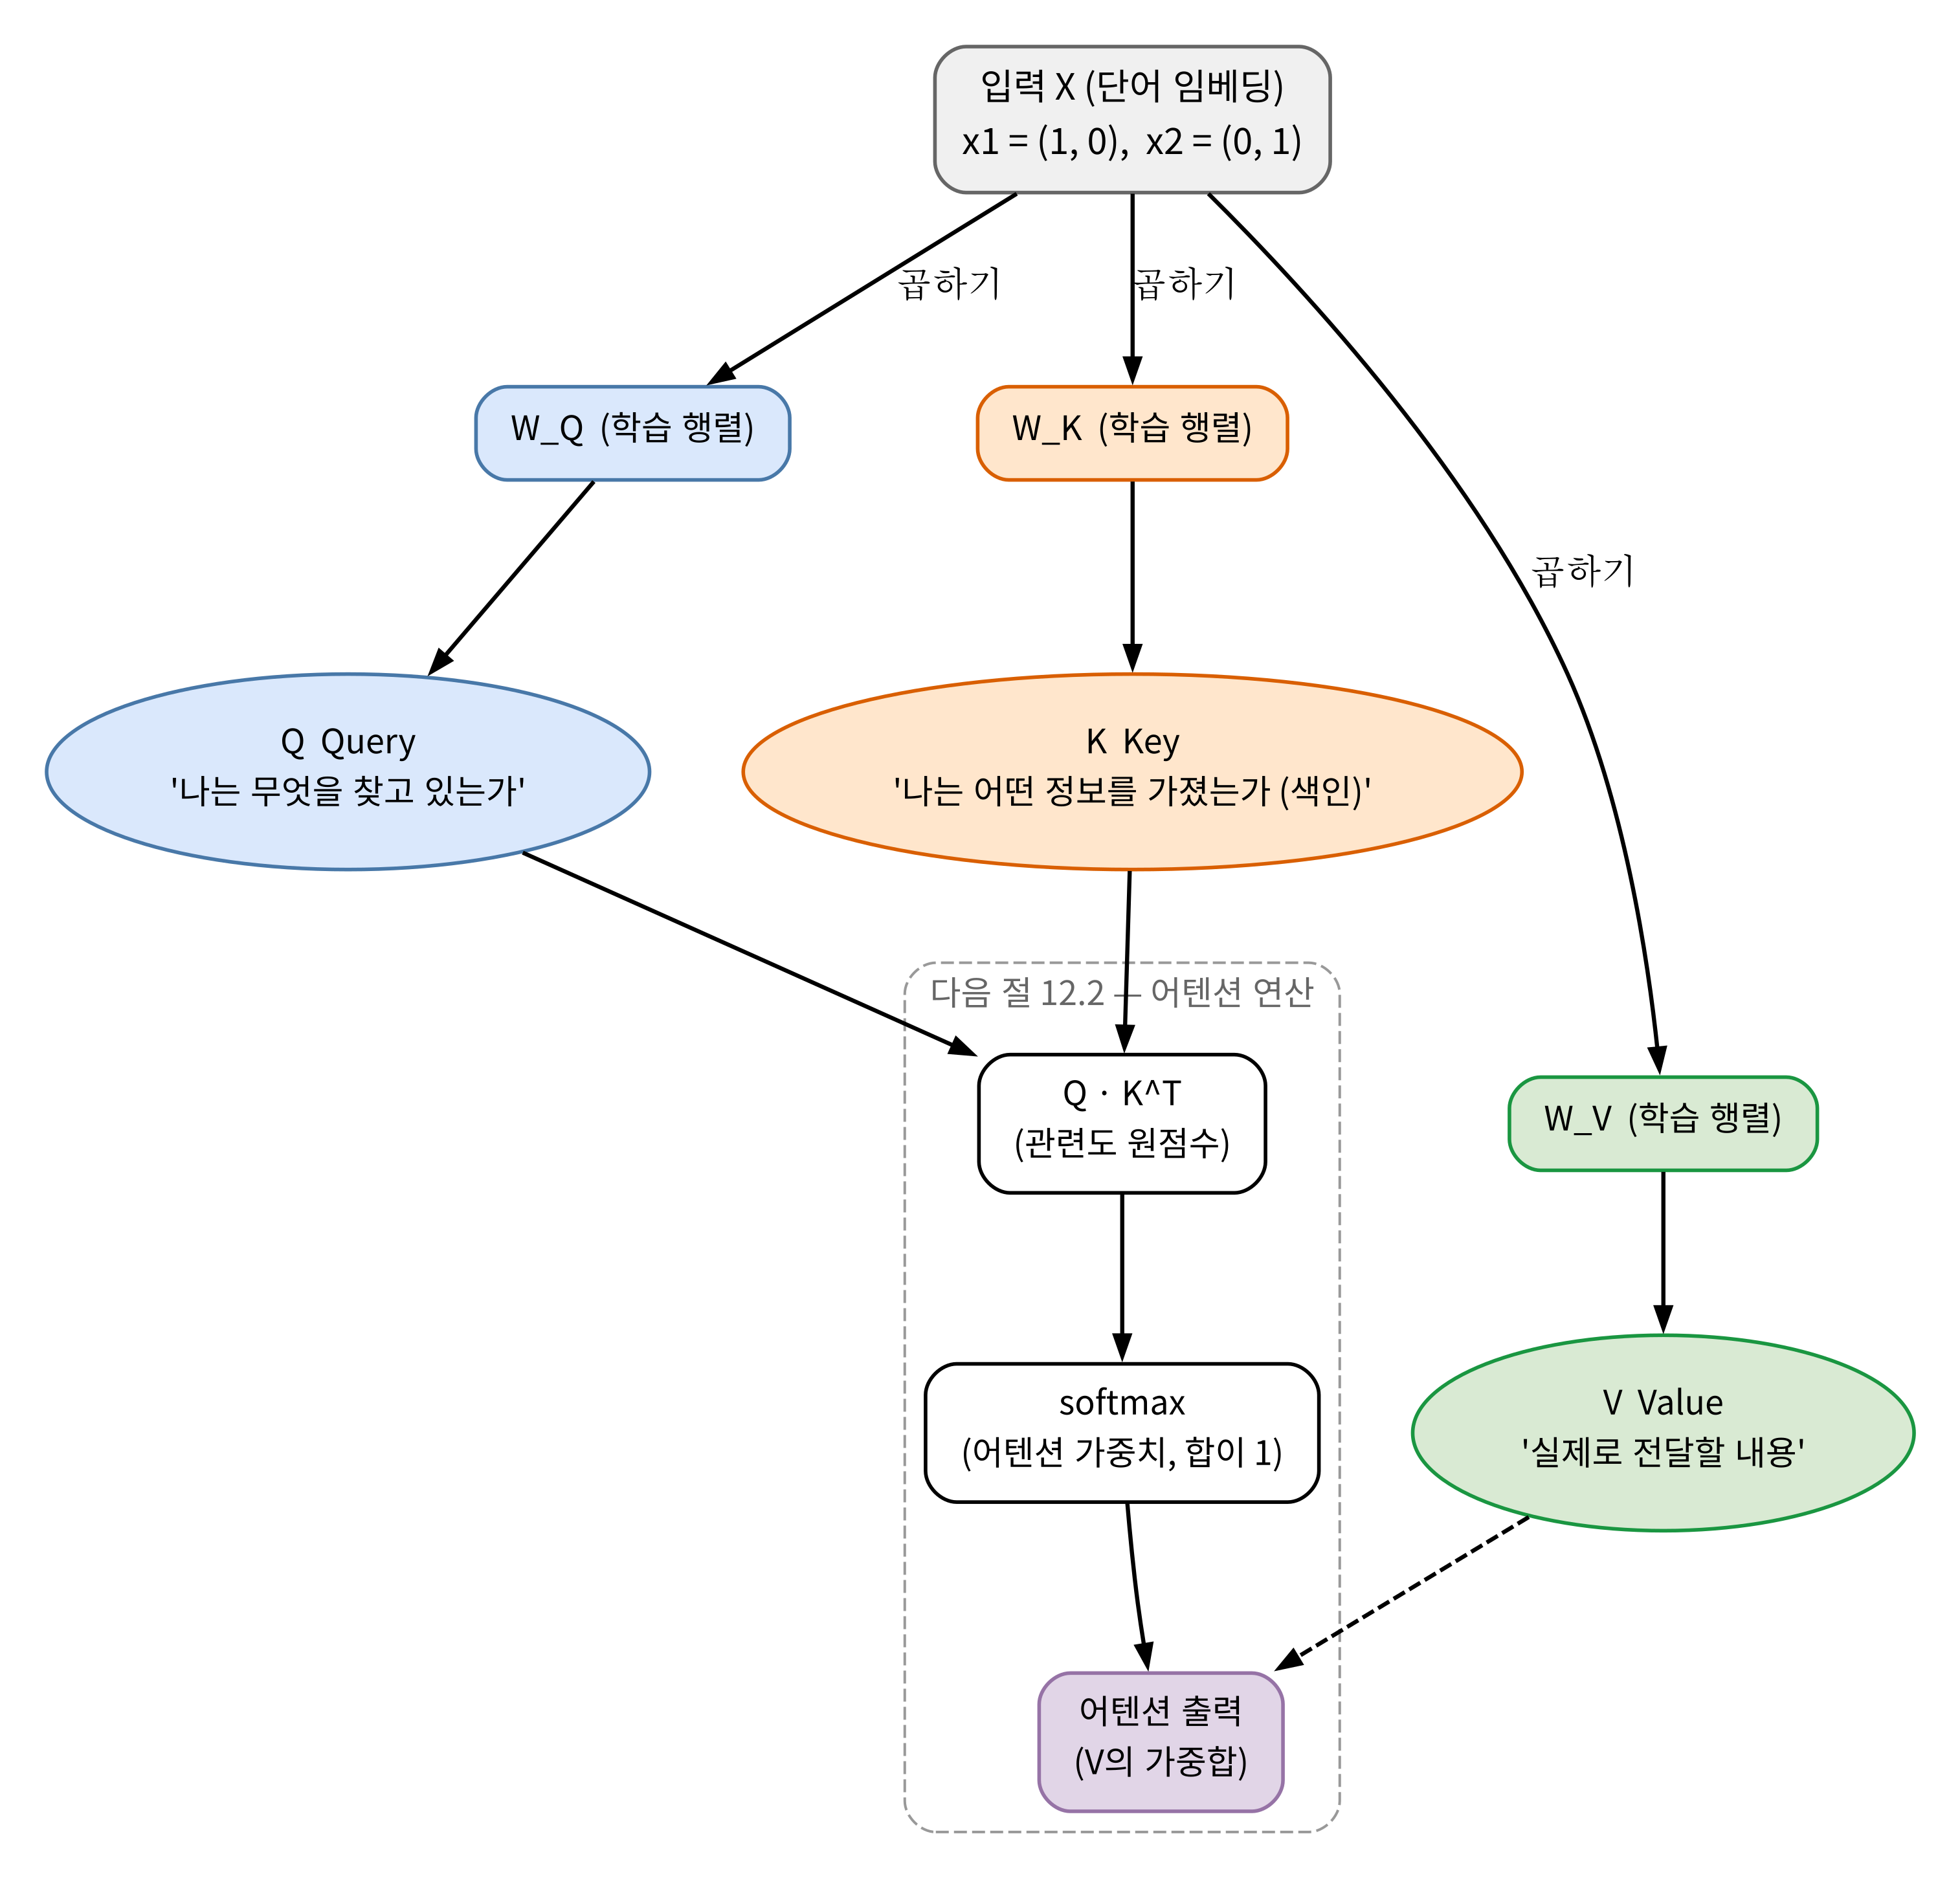
\includegraphics[width=\linewidth]{ch12_1_qkv.png}
      \vskip0.3em
      {\footnotesize 같은 입력 임베딩 $x_1, x_2$에 서로 다른 세 행렬
      $W_Q, W_K, W_V$ 를 곱해 Q·K·V를 만들고,
      $QK^T$ 점수 $\to$ softmax $\to$ $V$ 가중합으로 어텐션
      출력을 만든다.}
    \end{column}
  \end{columns}
\end{frame}

\begin{frame}{손으로 한 번: 같은 입력, 서로 다른 Q·K·V}
  단어 2개, 임베딩 $x_1=(1,0),\; x_2=(0,1)$ (즉
  $X=\begin{pmatrix}1&0\\0&1\end{pmatrix}$). 서로 다른 세 변환 행렬:
  \[W_Q=\begin{pmatrix}1&0\\0&2\end{pmatrix}, \quad
    W_K=\begin{pmatrix}0.5&0\\0&0.5\end{pmatrix}, \quad
    W_V=\begin{pmatrix}2&1\\1&2\end{pmatrix}\]
  $Q=XW_Q$, $K=XW_K$, $V=XW_V$ 를 계산하면:
  \[Q=\begin{pmatrix}1&0\\0&2\end{pmatrix}, \quad
    K=\begin{pmatrix}0.5&0\\0&0.5\end{pmatrix}, \quad
    V=\begin{pmatrix}2&1\\1&2\end{pmatrix}\]
  \vskip0.4em
  \begin{block}{핵심 관찰}
    같은 입력 $X$ 에서 출발했는데도 $Q, K, V$ 가 \textbf{서로 완전히
    다른 값}으로 나온다 — 세 행렬이 각각 \textbf{독립적인 학습
    파라미터}를 갖고 있기 때문이다.
  \end{block}
\end{frame}

\begin{frame}{세 행렬의 ``역할''은 학습이 만든다}
  2단어 예의 세 행렬이 각각 하는 일:
  \small
  \begin{tabular}{@{}llp{8cm}@{}}
    \toprule
    행렬 & 효과 & 역할 \\
    \midrule
    $W_Q$ & 두 번째 차원을 2배로 확대 & ``찾는 방향''을 세우다 \\
    $W_K$ & 모든 차원을 절반으로 축소 & ``색인''의 스케일을 줄이다 \\
    $W_V$ & 두 차원을 서로 섞음 (비대각 원소 $\neq 0$) &
      전달할 \textbf{내용}을 다른 공간에서 구성하다 \\
    \bottomrule
  \end{tabular}
  \vskip0.5em
  이렇게 서로 다른 ``역할''을 하는 변환들은 \textbf{학습을 통해
  만들어진다} — 사람이 ``이 행렬은 대명사 담당''이라고 설계하는
  것이 아니다.
  \vskip0.3em
  {\footnotesize 실습: \texttt{qkv(X, WQ, WK, WV)} 함수를 완성해
  손계산한 $Q, K, V$ 와 일치하는지 확인 — ``같은 입력에서 세 가지
  다른 결과''가 나옴이 이 절의 포인트.}
\end{frame}

\begin{frame}{왜 ``관련성''은 내적으로 재는가}
  12.2절에서 관련성은 \textbf{내적(dot product)}으로 잰다고 배운다.
  공식이 나오기 전에 ``왜 내적이냐''의 직관:
  \begin{itemize}
    \item 두 벡터의 내적 $a \cdot b = \|a\|\,\|b\|\,\cos\theta$ —
      \textbf{두 벡터의 방향이 얼마나 맞느냐}에 비례
      (노름을 나눠낸 $\cos\theta$ 가 곧 Ch.\,14.2의 코사인 유사도).
    \item 직각이면 0, 반대 방향이면 음수.
    \item ``찾는 정보의 방향'' = Query, ``가진 정보의 방향'' = Key 이면,
      \textbf{Q·K는 찾는 것과 가진 것의 방향이 일치할수록 큰 숫자}
      — ``관련성''의 정의 그 자체.
  \end{itemize}
  \vskip0.6em
  어텐션이 ``공간적 거리가 가까운가''(유클리드 거리)를 재는 게
  아니라 내적을 쓰는 이유: \textbf{``얼마나 가까운가''가 아니라
  ``얼마나 잘 맞는가(matching)''를 묻기} 때문.
  \vskip0.4em
  {\footnotesize 부수적 함의: 벡터 크기가 크면 내적이 자동으로
  커진다 — 12.2절이 $\sqrt{d_k}$ 로 스케일링하는 이유가 여기에도
  있다.}
\end{frame}

\begin{frame}{전체 파이프라인 미리보기: 3단계}
  위 2단어 예 하나로 12.2절의 ``어텐션 연산'' 전체를 미리 본다.
  \begin{enumerate}
    \item 모든 단어 쌍의 \textbf{원점수(raw score)} $QK^T$ 계산
    \item 각 행에 \textbf{softmax}를 적용해 분포(어텐션 가중치) 생성
    \item 그 가중치로 $V$ 의 행을 \textbf{가중합} $\to$ 출력
  \end{enumerate}
  \vskip0.6em
  원점수:
  \[QK^T = \begin{pmatrix} 1 & 0 \\ 0 & 2 \end{pmatrix}
  \begin{pmatrix} 0.5 & 0 \\ 0 & 0.5 \end{pmatrix}
  = \begin{pmatrix} 0.5 & 0 \\ 0 & 1 \end{pmatrix}\]
  \begin{itemize}
    \item 단어 1의 Query $(1,0)$: 단어 1의 Key $(0.5,0)$ 과 잘 맞고,
      단어 2의 Key $(0,0.5)$ 와는 직각(내적 0).
    \item 단어 2의 Query $(0,2)$: 자기 Key와 방향 일치
      ($2 \times 0.5 = 1$), 단어 1의 Key와는 0.
  \end{itemize}
  {\footnotesize 이 예에서는 $W_Q, W_K$ 를 각 단어가 서로를
  교차하지 않는 방향으로 \textbf{직접 설계}했다 — 실전에서는
  이 설계를 \textbf{학습}이 대체한다.}
\end{frame}

\begin{frame}{계산 이어가기: 스케일링·softmax·가중합}
  $\sqrt{d_k} = \sqrt{2}$ 로 나눈 뒤 각 행에 softmax:
  \begin{itemize}
    \item 행 1: softmax(0.354, 0) = \textbf{(0.587, 0.413)}
      \; (0.354 $= 0.5/\sqrt{2}$)
    \item 행 2: softmax(0, 0.707) = \textbf{(0.330, 0.670)}
      \; (0.707 $= 1/\sqrt{2}$)
  \end{itemize}
  \vskip0.5em
  최종 출력 ($V_1=(2,1), V_2=(1,2)$):
  \begin{itemize}
    \item 단어 1: $0.587\,V_1 + 0.413\,V_2 = \mathbf{(1.587,\ 1.413)}$
    \item 단어 2: $0.330\,V_1 + 0.670\,V_2 = \mathbf{(1.330,\ 1.670)}$
  \end{itemize}
  \vskip0.5em
  \begin{block}{두 가지 관찰}
    (1) \textbf{단어 1의 출력이 $V_1$ 쪽에, 단어 2의 출력이 $V_2$
    쪽에 기울어 있다} (0.59, 0.67) — ``관련 단어의 내용을 관련도만큼
    섞는다''가 숫자로 성립. (2) 출력이 순수한 복사
    (정답이면 (2,1)·(1,2))는 \textbf{아니다} — 다른 단어의 내용이
    조금 섞여 있다.
  \end{block}
  \vskip0.4em
  어텐션 출력은 ``가장 관련 있는 단어 \textbf{하나}를 고르는
  것''이 아니라 \textbf{``모든 Value의 가중평균''} — 이 체감이
  있으면 12.2절의 softmax가 ``\textbf{왜 합이 1인 분포}여야 하는
  지''가 자동으로 이해된다.
  \vskip0.3em
  \textbf{점수 차이가 클수록 어텐션 가중치는 더 집중}된다:
  단어 2의 점수 간격(1 vs 0)이 단어 1(0.5 vs 0)보다 크므로
  가중치도 더 기울어 있다 (0.67/0.33 vs 0.59/0.41). 어떤 Key의
  점수가 압도적으로 높으면 softmax는 가중치의 거의 전부를 거기에
  몰아넣는다 — 12.2절 실습의 ``그것은''이 ``동물''에 0.56을
  주는 현상은 바로 이 메커니즘의 \textbf{더 극단적인 버전}.
\end{frame}

\begin{frame}{A/B 비교: 변환 없이 Q=K=V=X로 쓰면}
  같은 2단어 예에서 \textbf{변환 없이} $Q = K = V = X$
  ($X=\begin{pmatrix}1&0\\0&1\end{pmatrix}$)로 어텐션을 돌려본다:
  점수 $XX^T = \begin{pmatrix}1&0\\0&1\end{pmatrix}$
  $\to$ $\sqrt{2}$ 스케일링 후 (0.707, 0) / (0, 0.707)
  $\to$ softmax 후 \textbf{(0.670, 0.330) / (0.330, 0.670)}
  $\to$ 출력: 단어 1 = (0.670, 0.330), 단어 2 = (0.330, 0.670).
  \vskip0.4em
  \small
  \begin{tabular}{@{}lll@{}}
    \toprule
    경우 & 어텐션 가중치 (단어 1 행) & 단어 1의 출력 \\
    \midrule
    $Q=K=V=X$ (변환 없음) & (0.670, 0.330) & (0.670, 0.330) \\
    학습된 $W_Q, W_K, W_V$ & (0.587, 0.413) & (1.587, 1.413) \\
    \bottomrule
  \end{tabular}
  \vskip0.4em
  \begin{center}
  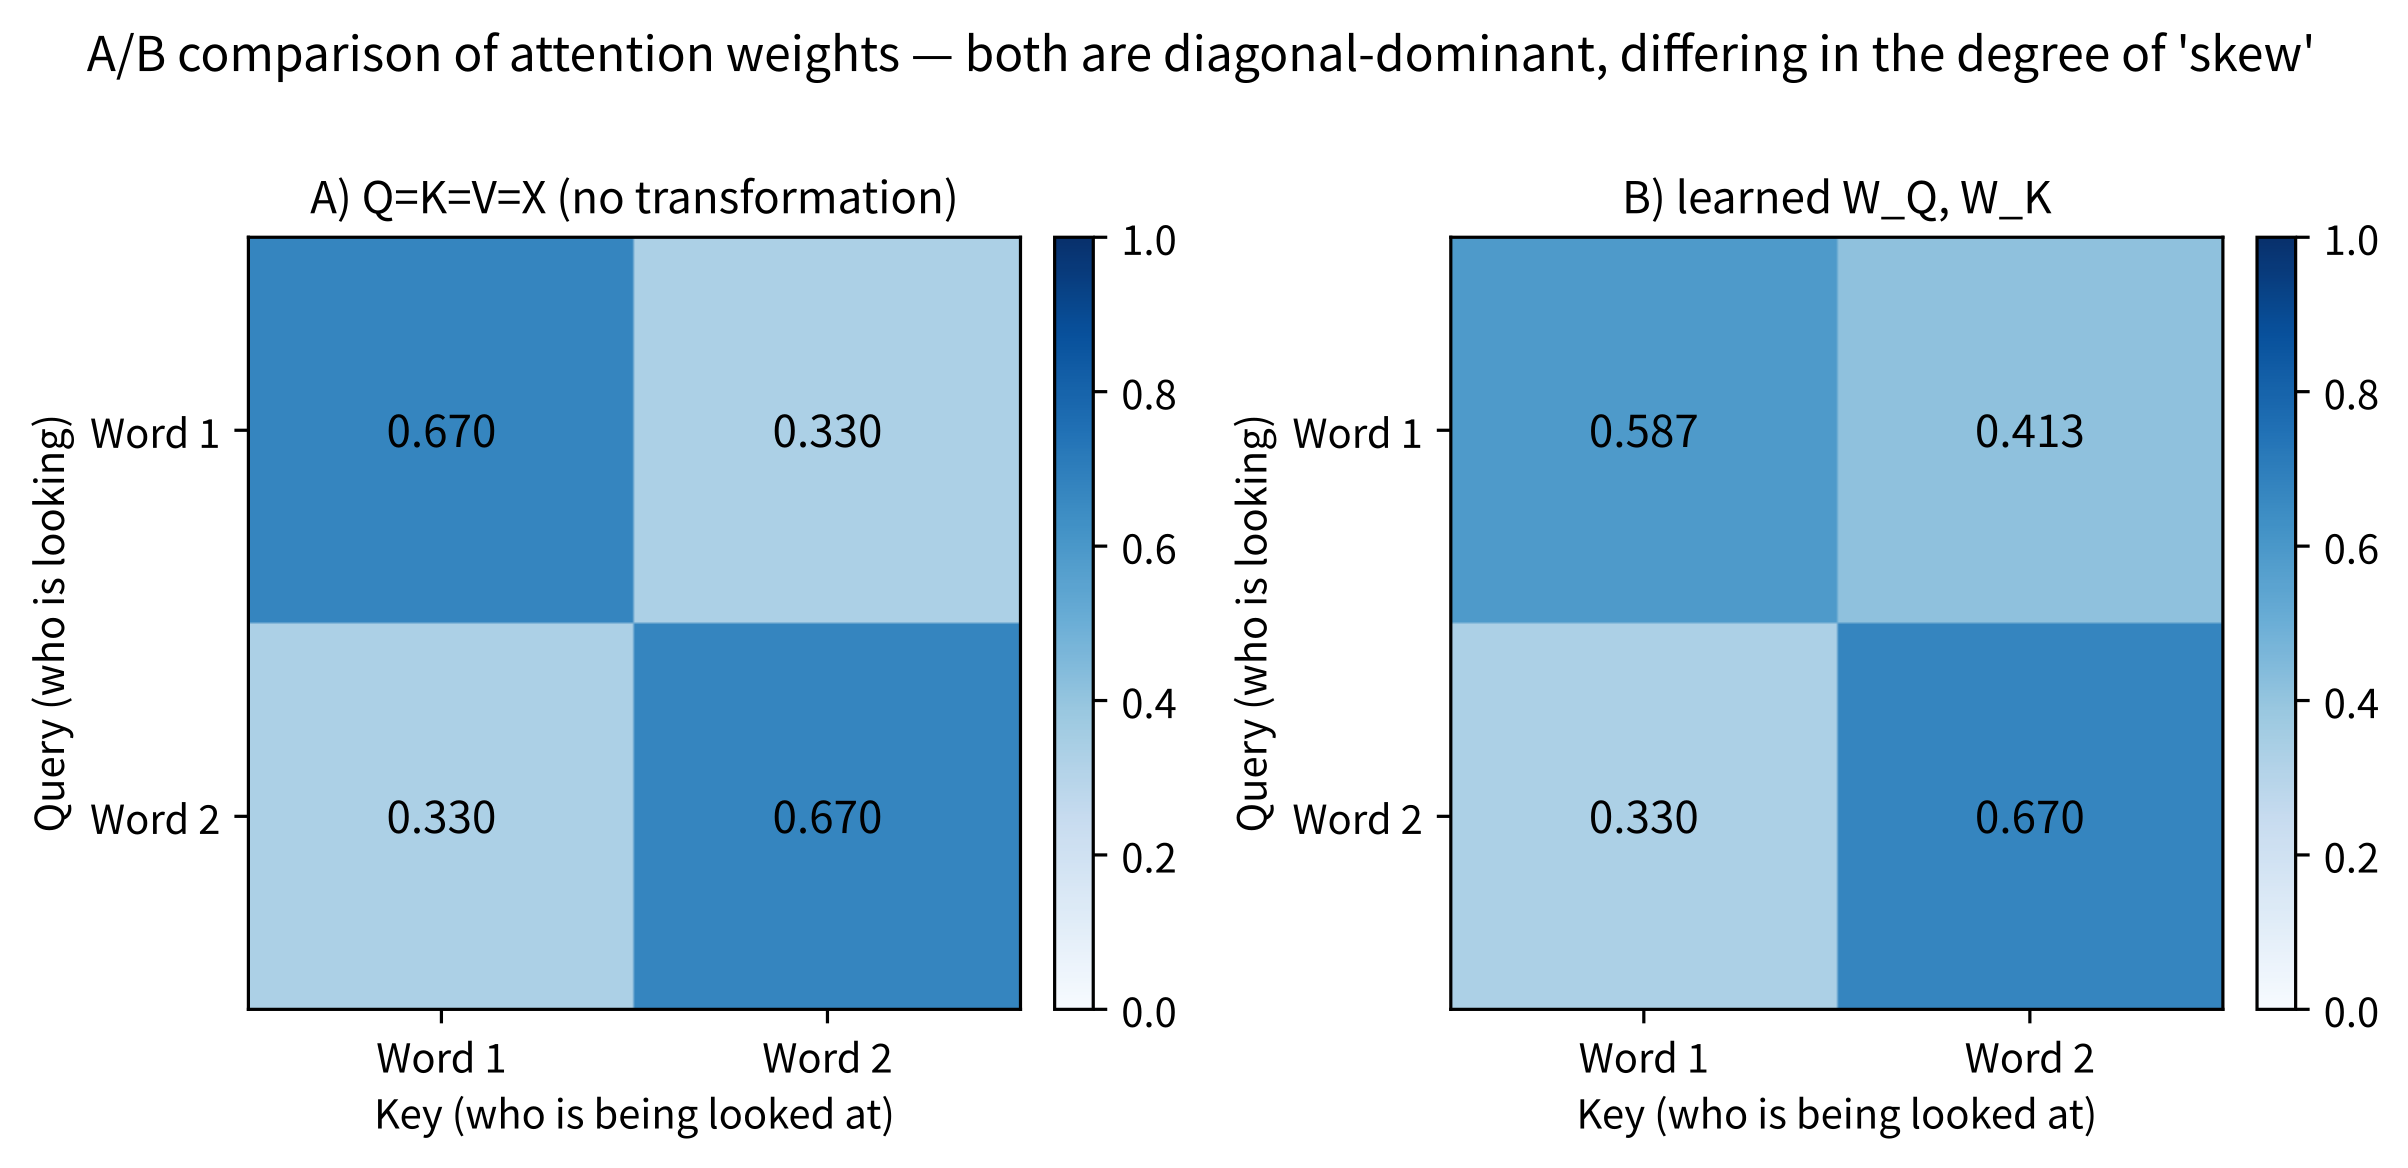
\includegraphics[width=0.6\linewidth]{ch12_1_qkv_weights.png}
  \end{center}
  {\footnotesize 두 경우 모두 대각선이 우세하지만 가중치의
  ``기울어짐'' 정도가 다르다.}
\end{frame}

\begin{frame}{변환이 없으면 두 가지가 깨진다}
  \begin{enumerate}
    \item \kb{자신의 임베딩과만 비게 된다.} 이 예의 임베딩이
      서로 직각인 단위 벡터이므로, 각 단어는 \textbf{자기 자신과만}
      높은 점수를 얻을 수밖에 없다 — 출력이 ``내 임베딩에 남의 것을
      약간 섞은 것''으로 고정된다.
    \item \kb{학습할 여지가 없다 (더 근본적).} $W_Q, W_K, W_V$ 는
      모델이 ``무엇을 찾고, 무엇으로 색인하고, 무엇을 전달할지''를
      데이터로부터 배울 수 있는 \textbf{유일한} 자리다.
  \end{enumerate}
  \vskip0.5em
  처음부터 $Q=K=V=X$ 로 고정하면 데이터에 무엇을 더 넣어도
  어텐션 구조는 변하지 않는다 — \textbf{``데이터가 구조를
  결정''할 틈이 없는 고정 템플릿}과 같다.
  \vskip0.4em
  \begin{block}{핵심}
    기울기가 실제로 흘러 $W_Q, W_K, W_V$ 가 갱신되는 부분이 곧
    모델이 ``어떤 관계를 보게 될지''를 결정하는 부분이다 —
    이 세 행렬의 존재가 어텐션 메커니즘의 \textbf{핵심}.
  \end{block}
\end{frame}

\begin{frame}{자주 묻는 질문 1: 왜 세 가지로 나뉘나}
  \kq{Q·K·V는 왜 같은 입력에서 서로 다른 세 가지로 나뉘나요?
  입력 자체를 비교하면 안 되나요?}
  \begin{itemize}
    \item $Q=K=V=X$ (변환 없이 원본 입력을 그대로 씀)라면
      ``이 단어가 자기 자신과 얼마나 비슷한가''만 재게 되어
      \textbf{표현력이 크게 제한}된다.
    \item 서로 다른 학습 가능한 변환 $W_Q, W_K, W_V$ 를 두면,
      ``무엇을 찾을지''와 ``무엇을 제공할지''를 모델이
      \textbf{데이터로부터 독립적으로 학습}할 수 있다.
    \item 예: 대명사는 ``나를 가리키는 명사를 찾는다'' 방향으로
      $W_Q$ 가, 명사는 ``대명사가 찾는 대상이 될 수 있다'' 방향으로
      $W_K$ 가 학습된다.
  \end{itemize}
  \vskip0.5em
  {\footnotesize 보충: ``내적(유사도)으로 관련을 재고, 학습된 변환을
  거친 뒤 비교한다''는 패턴은 Ch.\,5.3 커널 함수 $K(x,x')$ 과
  정신적으로 닮아 있다.}
\end{frame}

\begin{frame}{자주 묻는 질문 2: Q와 K가 중복되는 것 아닌가}
  \kq{Q, K가 같은 X에서 나오는데, 출력이 ``X를 하나의 행렬로
  변환한 것''과 같지는 않나요?}
  \begin{itemize}
    \item \textbf{중복이 아니다.} 점수 $QK^T$ 는 \textbf{두 행렬의
      곱}으로 결정된다 — 같은 $X$ 여도 $W_Q$ 와 $W_K$ 가 무엇이냐에
      따라 ``어떤 단어 쌍이 만나고 어떤 쌍이 안 만나는지''가
      완전히 달라진다.
    \item 같은 $X$ 를 ``질문 카드·색인 카드·내용 카드'' 세 장으로
      찍어 내는 것과 같다 — 질문·색인 카드는 \textbf{비교 단계}에서만,
      내용 카드는 \textbf{전달 단계}에서만 쓰인다.
    \item $Q=K$ 로 고정하면 $QK^T$ 가 \textbf{대칭}이 되어
      ``내가 너를 찾는 정도'' = ``너가 나를 찾는 정도''가 되어
      \textbf{비대칭적 관계}를 표현할 수 없다.
  \end{itemize}
  \vskip0.4em
  예: ``대명사는 명사를 찾지만, 명사는 대명사를 찾지 않는다'' —
  실제 모델에서 어텐션의 \textbf{방향성}(어떤 헤드는 뒤쪽, 어떤
  헤드는 앞쪽 단어를 본다)은 바로 이 \textbf{비대칭성}에서 나온다.
  \vskip0.3em
  \kq{그렇다면 왜 편항(bias)이 아니라 \textbf{행렬 곱}인가?}
  \begin{itemize}
    \item 편항은 모든 단어에 \textbf{같은} 벡터를 더하는 것 —
      ``단어 A는 대명사고 단어 B는 명사''를 구분할 수 없고,
      단어 사이의 \textbf{상대적 기하학}(각도, 방향)이 그대로다.
    \item 내적 점수는 바로 그 상대적 기하학으로 결정된다 —
      점수의 의미를 바꾸려면 방향 자체를 돌리거나 늘리거나 섞을 수
      있어야 한다(선형 변환). 선형만으로는 공간을 ``접을'' 수 없다
      (Ch.\,9.2) — 어텐션에서는 그 ``접는 역할''을
      \textbf{점수 비교}가 대신 맡는다.
  \end{itemize}
\end{frame}

\begin{frame}{자주 묻는 질문 4: 실제 모델에서 얼마나 큰가}
  2017년 원논문(Vaswani et al.)의 스케일:
  \begin{itemize}
    \item 모델 차원 $d_{model} = 512$ $\Rightarrow$ $W_Q, W_K, W_V$ 는
      각각 \textbf{512$\times$512} 행렬 (각각 약 \textbf{26만}개
      파라미터).
    \item 감각 비교: Ch.\,6 당뇨 회귀 문제가 특징 10개인 것과
      비교하면 스케일을 잡기 좋다.
    \item 12.3절 멀티헤드에서는 이 512차원을 $h=8$ 개 헤드에 나눠
      쓰므로 각 헤드 행렬은 \textbf{64$\times$64}가 된다.
  \end{itemize}
  \vskip0.6em
  세 행렬 모두 \textbf{학습으로 결정}된다 — 사람이 ``이 행렬은
  대명사 담당''이라고 설계하지 않는다.
  \vskip0.4em
  12.3절에서 보듯, 헤드들이 각자 다른 역할로 \textbf{스스로 분화}
  한다는 것을 숫자와 관측으로 확인한다.
\end{frame}

\begin{frame}{자주 하는 실수: ``검색'' 단계를 건너뛰기}
  \kq{어텐션을 ``가중평균''으로만 보고 관련도 계산(3단계의
  중간)을 건너뛰는 것.}
  \begin{itemize}
    \item 처음 접할 때 가장 흔한 오해: 3단계의 중간 —
      \textbf{관련도 계산} — 을 건너뛰고 ``$V$ 의 가중평균''만
      기억해 두는 것.
    \item $V$ 의 어떤 행이 많이 섞이게 될지를 결정하는 것은
      \textbf{점수($QK^T$)}이며, $V$ 가 아니라 \textbf{$W_Q, W_K$ 가}
      그 점수를 만든다.
    \item \textbf{$V$ = ``무엇을 mix할지'', 점수 = ``얼마나
      mix할지''.} 점수가 엉뚱하면 $V$ 의 가중평균은
      \textbf{무관한 단어들의 평균}이 된다.
  \end{itemize}
  \vskip0.5em
  구현하거나 학습된 모델의 어텐션을 디버깅할 때 첫 단계는 항상
  \textbf{점수 행렬의 패턴을 보는 것}:
  \begin{itemize}
    \item 대각선이 압도적으로 큰가 (각 단어가 \textbf{자기 자신만}
      보는 패턴)
    \item 특정 열이 압도적인가 (많은 단어가 하나의 단어를 보고 —
      ``그것은''의 ``동물''처럼 \textbf{중심어}가 끌어당기는 경우)
    \item 거의 균일한가 (\textbf{집중 실패} — 가중치 행렬이 역할을
      찾지 못했거나, 임베딩이 서로 구별이 안 되는 상태)
  \end{itemize}
\end{frame}

% ===== SECTION 12.2 =====
\section{12.2 스케일드 닷-프로덕트 어텐션과 셀프-어텐션}
\begin{frame}{트랜스포머 원논문의 핵심 연산}
  \begin{columns}[T]
    \begin{column}{0.44\textwidth}
      \centering
      
\includegraphics[width=\linewidth]{ref_transformer.png}
      \vskip0.3em
      {\footnotesize 트랜스포머 전체 구조 — 인코더(왼쪽)와 디코더
      (오른쪽)의 Multi-Head Attention + Feed Forward 스택
      (Vaswani et al., 2017, Figure 1).}
    \end{column}
    \begin{column}{0.52\textwidth}
      \kb{Scaled dot-product attention}은 Transformer 원논문의
      핵심 연산. 한 단어의 Query가 모든 단어의 Key와 얼마나
      ``관련 있는가''를 내적(dot product)으로 잰다 (Bahdanau et
      al., 2014; Luong et al., 2015):
      \[
      \text{Attention}(Q, K, V) =
      \text{softmax}\left(\frac{QK^T}{\sqrt{d_k}}\right)V
      \]
      \vskip0.4em
      $d_k$ = Key 벡터의 \textbf{차원} (12.2 말미 실수 섹션 참고).
    \end{column}
  \end{columns}
\end{frame}

\begin{frame}{4단계로 뜯어보기}
  \begin{enumerate}
    \item \kb{$QK^T$} — 모든 단어 쌍의 Query-Key 내적을 \textbf{한
      번에} 계산한 행렬. 각 행 = 한 단어가 다른 모든 단어와
      얼마나 관련 있는지에 대한 \textbf{원점수}.
    \item \kb{$\sqrt{d_k}$ 로 나누기} (Key 벡터 차원의 제곱근) —
      내적값이 차원이 커질수록 커지는 경향이 있어, softmax가
      극단적인 값(0 또는 1에 가까운)만 내뱉게 되는 것을 막는
      \textbf{스케일 조정}.
    \item \kb{softmax} — 각 행을 \textbf{확률분포}(합이 1)로
      바꿈. ``이 단어가 다른 단어들에게 나눠 주는 주의의 비율''.
    \item \kb{$V$ 가중합} — 그 확률로 $V$(각 단어가 실제로
      전달할 내용)의 가중합을 냄. 결과 = \textbf{``관련 단어들의
      내용을 관련도만큼 섞어 담은''} 새로운 벡터.
  \end{enumerate}
\end{frame}

\begin{frame}[fragile]{코드로 4단계}(실습)
\begin{lstlisting}
import math

def softmax(row):
    m = max(row)
    exps = [math.exp(v - m) for v in row]
    total = sum(exps)
    return [e / total for e in exps]

def attention(Q, K, V, d_k):
    scores = [[sum(Q[i][t] * K[j][t] for t in range(d_k))
               / math.sqrt(d_k) for j in range(len(K))]
              for i in range(len(Q))]          # QK^T / sqrt(d_k)
    weights = [softmax(row) for row in scores] # softmax
    output = [[sum(weights[i][j] * V[j][t] for j in range(len(V)))
               for t in range(len(V[0]))]
              for i in range(len(Q))]          # V 가중합
    return output, weights
\end{lstlisting}
  {\footnotesize 실전에서는 이 4단계를 numpy 행렬 곱으로 한 줄씩
  줄인다 (실습 노트북 참고).}
\end{frame}

\begin{frame}{코드 읽기: 4단계가 그대로 번역}
  \begin{itemize}
    \item \texttt{scores[i][j]} = $Q[i] \cdot K[j] / \sqrt{d_k}$ —
      $QK^T$ 의 $(i,j)$ 성분. \texttt{scores} 전체가 $n \times n$
      \textbf{원점수 행렬} 자체.
    \item \texttt{weights[i]} = \texttt{scores[i]}에 softmax를
      적용한 결과 — $i$번째 단어(행)가 $j$번째 단어들(열)에
      나눠준 주의의 비율, \textbf{합이 1}.
    \item \texttt{output[i]} = \texttt{weights[i]}라는 가중치로
      $V$ 의 $n$개 행을 \textbf{가중합}한 값 — ``$i$번째 단어가
      다른 단어들에게 요청한 정보(V)들을 관련도만큼 섞은 결과''.
  \end{itemize}
  \vskip0.5em
  3중 중첩 리스트 컴프리헨션이 처음엔 눈에 거슬리겠지만,
  각각 $QK^T$ $\to$ $\sqrt{d_k}$ 스케일 $\to$ softmax $\to$
  $V$ 가중합의 4단계를 \textbf{그대로 번역}한 것일 뿐이다.
\end{frame}

\begin{frame}{softmax를 다시 볼 이유: 차이를 증폭}
  Ch.\,2.3(로지스틱 회귀의 출력을 확률로), Ch.\,3(합이 1인
  분포)에서 만난 softmax가, 어텐션 맥락에서 더 예리하게 —
  \kq{\textbf{원점수 간 ``차이''를 지수적으로 증폭}한다.}
  \vskip0.4em
  \textbf{2개 단어의 가장 단순한 경우} ($s_1=0$, $s_2=g$):
  \[p_2 = \frac{e^{g}}{1 + e^{g}} = \frac{1}{1 + e^{-g}}
      = \sigma(g)\]
  \textbf{어텐션 원점수 차이에 대한 softmax는 정확히 시그모이드
  $\sigma(g)$} — 로지스틱 회귀의 결정 함수가 ``원점수
  \emph{차이}''를 입력으로 받는 모습. 두 원점수 사이의 ``차이''
  크기가 가중치의 극단적 정도를 사실상 \textbf{단독으로}
  결정한다:
  \small
  \begin{tabular}{@{}lll@{}}
    \toprule
    원점수 차이 $g$ & 가중치 $(p_1, p_2)$ & 해석 \\
    \midrule
    0.5 & (0.378, 0.622) & 아직 균형 \\
    2 & (0.119, 0.881) & 한쪽 우세 \\
    8 & (0.0003, 0.9997) & 사실상 하드 선택 \\
    \bottomrule
  \end{tabular}
  \vskip0.4em
  차이가 0.5에서 8로 \textbf{16배}가 되자 ``62:38의 균형''이
  ``99.97:0.03의 독주''로. 원점수가 큰 차원의 내적(차원에 비례해
  커짐)을 그대로 넣으면 \textbf{거의 one-hot} — ``관련 단어
  \emph{하나}만 고르는'' 하드 경로가 되어 (1) \textbf{선택된
  단어의 가중치 미분이 0}(학습 신호 끊김), (2) \textbf{원점수
  미세 변화에 가중치가 급격히 뒤집혀} 불안정.
  $\sqrt{d_k}$ 스케일링은 이 \textbf{``softmax의 극단화''를 막는
  안전장치}.
\end{frame}

\begin{frame}{$\sqrt{d_k}$로 나누는 이유: 분산의 정수학}
  \textbf{``내적값이 차원이 커질수록 커진다''는 정확히 무엇을
  뜻하는가?}
  \begin{itemize}
    \item $q = (q_1, \dots, q_{d_k})$, $k = (k_1, \dots, k_{d_k})$
      가 서로 독립이고 각 성분이 \textbf{평균 0·분산 1}의 분포에서
      나온 벡터라고 하자.
    \item 내적 $\sum_{t=1}^{d_k} q_t k_t$ 는 \textbf{독립한 0평균
      곱 $d_k$개의 합}.
    \item 각 항 $q_t k_t$ 의 분산은 1 (독립 0평균·분산 1 변수 두
      개의 곱)이고, 독립 변수의 합은 \textbf{분산이 더해진다}.
  \end{itemize}
  \[
  \mathbb{E}[q \cdot k] = 0, \qquad
  \text{Var}[q \cdot k] = d_k
  \quad \Longrightarrow \quad
  \text{표준편차} = \sqrt{d_k}
  \]
  \vskip0.3em
  즉 \textbf{스케일링하지 않은 내적은 $\sqrt{d_k}$ 스케일로
  ``자라난다''} — 차원 64이면 표준편차 약 8, 차원 512이면 약 23.
  원점수가 $\pm 20 \sim 30$ 스케일로 벌어지면, softmax는 one-hot에
  붙어버린다.
\end{frame}

\begin{frame}{실제로 재보기: 무작위 내적 200쌍}
  \begin{columns}[T]
    \begin{column}{0.5\textwidth}
      무작위 벡터(각 성분 $\mathcal{N}(0,1)$) 두 개를 200쌍
      만들어 내적 계산 ($d=64$):
      \small
      \begin{tabular}{@{}ll@{}}
        \toprule
        & 관측 범위 \\
        \midrule
        스케일링 \textbf{전} & $-19.1 \sim +22.3$ \\
        $\sqrt{64} = 8$으로 \textbf{후} & $-2.4 \sim +2.8$ \\
        \bottomrule
      \end{tabular}
      \vskip0.4em
      \begin{itemize}
        \item 최대치 22.3 $\approx 2.8\sigma$ — \textbf{기대와
          일치}.
        \item \emph{전}의 $-19 \sim +22$면 softmax는 사실상
          one-hot ($\sigma(22) \approx 1 - 2.7 \times 10^{-10}$).
        \item $\sqrt{64} = 8$으로 나누면 \textbf{$-2.4 \sim +2.8$} —
          ``분화된 가중치''를 정상적으로 내는 범위.
      \end{itemize}
      $\sqrt{d_k}$ 는 ``마법 숫자''가 아니라 \textbf{내적의
      표준편차를 정확히 1로 되돌리는 상수} — ``무작위 기준선''에서
      얼마나 벗어났는지를 \emph{표준편차 단위로} 재게 한다.
    \end{column}
    \begin{column}{0.46\textwidth}
      \centering
      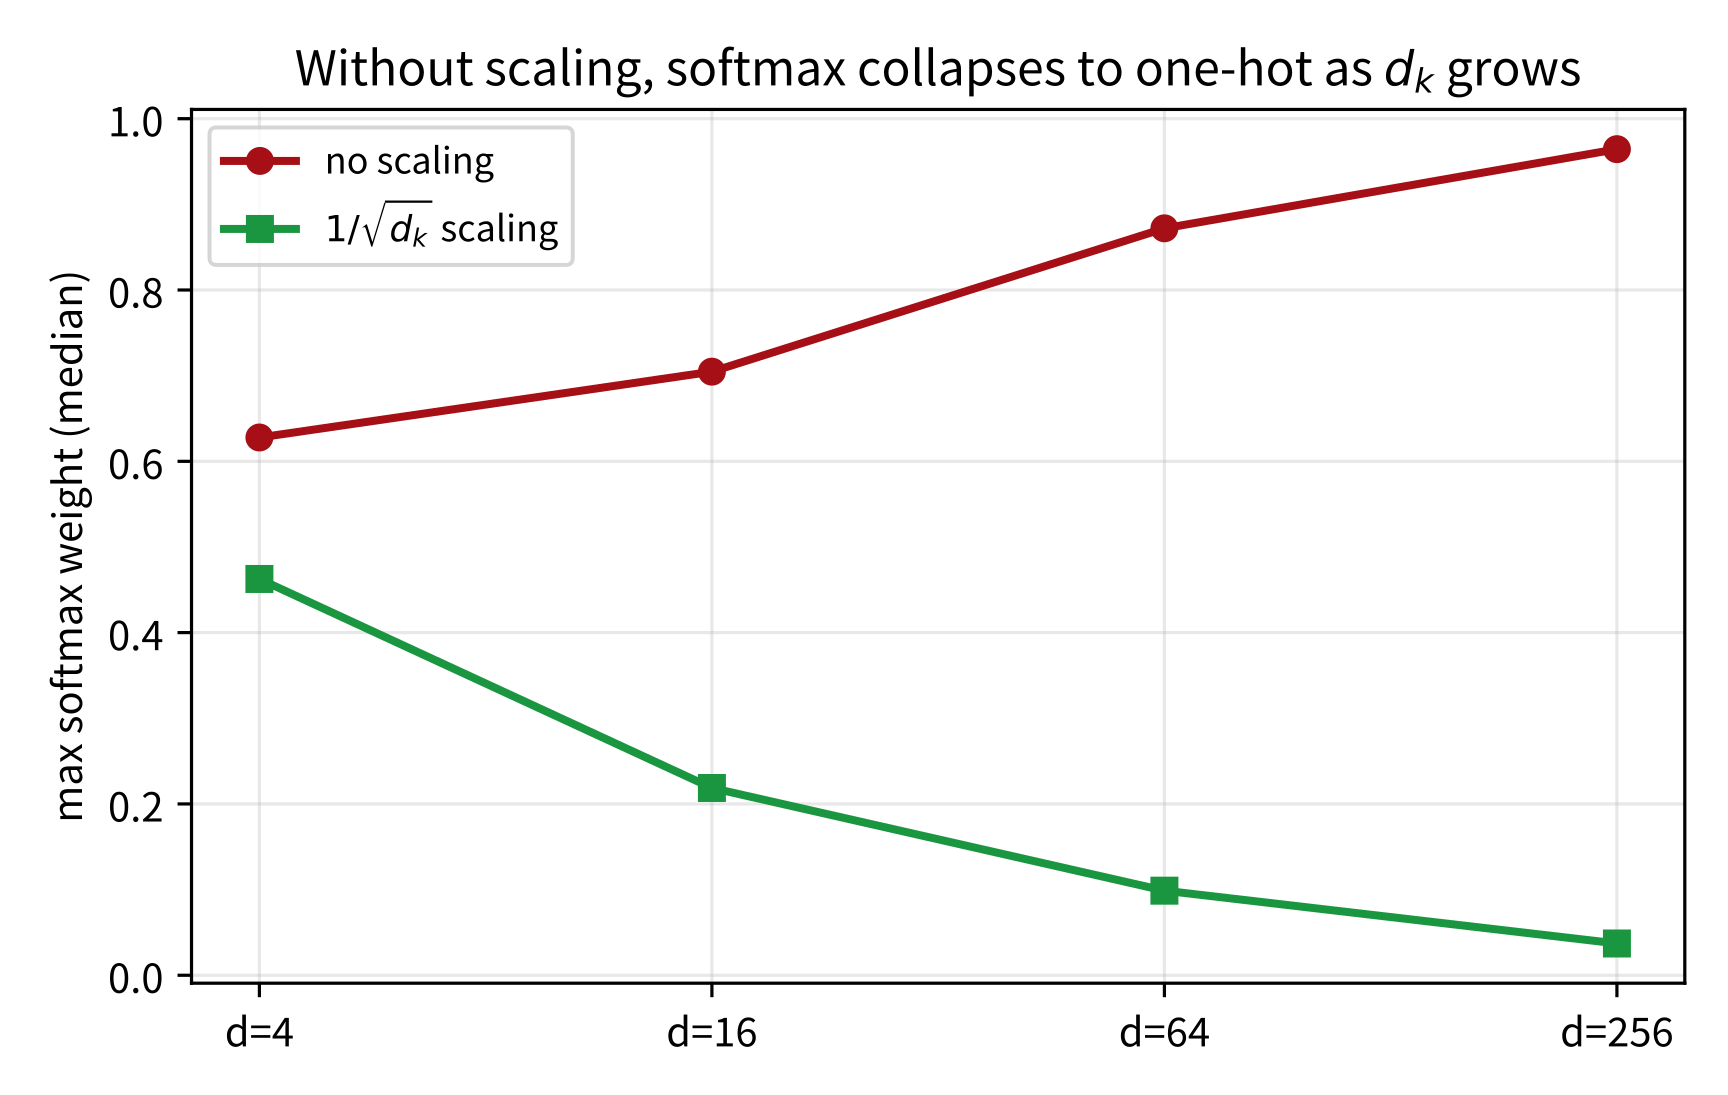
\includegraphics[width=\linewidth]{ch12_2_scaling_vs_dim.png}
      \vskip0.3em
      {\footnotesize 차원 $d_k$ 가 커질 때, 스케일링 없이
      $d$: 4$\to$256이면 softmax \textbf{최대 가중치 0.63$\to$0.96}
      (one-hot에 수렴); $1/\sqrt{d_k}$ 스케일링은 $d$와 무관하게
      \textbf{0.46$\to$0.04}로 낮게(분화되게) 유지 (500회 평균,
      실습 실험 6).}
    \end{column}
  \end{columns}
  \vskip0.5em
  $\sqrt{d_k}$ 가 ``차원을 모르는 마법 상수''가 아니라
  \textbf{``내적의 표준편차를 1로 환원하는'' 스케일}이라,
  원점수가 \emph{의미 있는 차이}를 가질 때 softmax가
  \emph{어떤 차원이든} 정상적으로 분화된다.
\end{frame}

\begin{frame}{온도(temperature) 관점}
  \kq{``$\sqrt{d_k}$ 가 아니라 $d_k$ 로 나누면 안 되나?''}
  \begin{itemize}
    \item $d_k$ 로 나누면 내적의 표준편차가 $1/\sqrt{d_k}$ 까지
      \textbf{과도하게} 줄어든다 — 원점수가 모두 0에 붙어
      softmax가 \textbf{균등분포}$(1/n)$에 가까워지고, ``어떤
      단어가 관련 있는가'' 구분하는 신호가 소실된다.
    \item 스케일링은 ``\textbf{정확히} 정규화''의 문제 —
      $\sqrt{d_k}$ 가 아니라 $d_k$ 나 1이면 softmax 출력이
      극단(one-hot)이나 반대(균등)로 치우친다.
    \item 실습 노트북에서 세 가지 스케일 ($1$, $\sqrt{d_k}$,
      $d_k$)을 같은 원점수에 적용해 가중치 분포를 나란히 비교.
  \end{itemize}
  \vskip0.5em
  \begin{block}{더 일반적인 형태: 온도 $t$}
    어텐션 원점수를 온도 $t$ 로 나눠 $\text{softmax}(s/t)$ 로
    적용. $t$ 크면 가중치가 \textbf{균등에 가까워지고}, $t$ 작으면
    \textbf{극단적}(한 단어 독주). $\sqrt{d_k}$ 스케일링은 초기
    무작위 상태에서 원점수의 표준편차가 $\sqrt{d_k}$ 라는 사실을
    이용해 \textbf{$t = \sqrt{d_k}$ 라는 ``정규 온도''}를 선택한
    것. 실전에서 이 온도 관점으로 어텐션을 의도적으로
    ``분산''/``집중''하게 조절하기도 한다.
  \end{block}
\end{frame}

\begin{frame}{실습: 원점수 2개만 있는 예로 흐름 추적}
  $n=2$, $d_k=2$ 아주 작은 예. $Q = K = \begin{pmatrix}1&0\\0&1\end{pmatrix}$,
  $V = \begin{pmatrix}10&0\\0&10\end{pmatrix}$.
  \begin{enumerate}
    \item \kb{Step 1 — $QK^T$}: 항등행렬이므로
      $QK^T = \begin{pmatrix}1&0\\0&1\end{pmatrix}$.
      (1,1) 성분 $= 1 \times 1 + 0 \times 0 = 1$.
    \item \kb{Step 2 — $\sqrt{d_k} = \sqrt{2} \approx 1.414$ 로
      나누기}: $\dfrac{QK^T}{\sqrt{2}} =
      \begin{pmatrix}0.707&0\\0&0.707\end{pmatrix}$.
    \item \kb{Step 3 — 첫 행 $[0.707, 0]$ 에 softmax}:
      $e^{0.707} \approx 2.028$, $e^0 = 1$, 합 3.028.
      \[p_1 = \frac{2.028}{3.028} \approx 0.670, \qquad
        p_2 = \frac{1}{3.028} \approx 0.330\]
      첫 단어는 \emph{자기 자신}에 67\%, 다른 단어에 33\% —
      Q·K가 \emph{같은} 벡터라 \textbf{자기 비교가 항상 한 번
      더 유리한 구조}(아래 ``자기 주입'' 참고).
    \item \kb{Step 4 — 가중합}:
      $\text{out}_1 = 0.670 \times V_1 + 0.330 \times V_2 =
      (6.70, 3.30)$.
  \end{enumerate}
  \vskip0.4em
  출력 $(6.70, 3.30)$ 을 $V$ 의 원행들 $(10,0), (0,10)$ 과
  비교하면 \textbf{첫 번째 $V$ 에 67\%의 ``분량''이 더
  섞여 있다}는 것이 직접 보인다 — ``관련도가 높은 단어의
  Value가 더 많이 기여한다''는 어텐션의 \textbf{핵심 행동}이
  숫자로 구현된 모습. (이 예는 12.3절 연습문제 3의 설정과
  정확히 같다.)
  \vskip0.3em
  \begin{block}{핵심 한 줄}
    ``관련 단어의 내용을 관련도만큼 섞는다'' — 이 문장이
    $QK^T \to$ 스케일링 $\to$ softmax $\to$ $V$ 가중합의
    4단계를 통과하면서 숫자가 되는 과정이다.
  \end{block}
\end{frame}

\begin{frame}{어텐션 출력의 볼록성: 볼록 껍질 안에만 존재}
  마지막 단계(가중합)가 \textbf{가중치의 합이 1인 가중 평균}이라는
  사실은 출력의 \emph{범위}에 강한 제약을 준다:
  \begin{itemize}
    \item 각 출력 $o_i = \sum_j w_{ij} v_j$ ($\sum_j w_{ij} = 1$,
      $w_{ij} \ge 0$)은 \textbf{$V$ 의 원행들의 볼록 결합}
      $\Rightarrow$ $V$ 원행들로 만드는 \textbf{볼록 껍질
      (convex hull) 안에 항상 존재}.
    \item \textbf{네 단어 예 숫자로 확인}: ``동물''의 출력
      $[2.898, 0.133, 0.010]$ — $V$ 원행(= $E$ 의 원행)들의
      범위가 각 차원 0$\sim$3인데, 각 성분은 모두 0$\sim$3 안에
      있고 \textbf{성분 합도 3.041로 $V$ 원행의 성분 합 (= 3)과
      거의 같}다. ``균등 어텐션''(모두 1/4)의 출력은 단순 평균
      $[1.45, 0.825, 0.75]$ 로, 실제 출력과는 \emph{완전히
      다른} 벡터 — 가중치가 ``분포''에 따라 출력은 볼록 껍질
      안에서 \emph{아무 위치나} 만들 수 있다.
  \end{itemize}
  \vskip0.4em
  \begin{block}{실전에서 이어지는 두 가지}
    (1) \textbf{출력의 스케일이 입력 스케일의 범위 안에 갇혀
    있다} — $V$ 가 큰 값으로 학습되면 출력도 그 범위 안에서만
    ``미세 조정'' (때로는 \emph{장점 — 안정성}, 때로는
    \emph{한계} — ``$V$ 가 표현할 수 없는 값''은 한 층으로
    만들 수 없음). (2) \textbf{가중치가 극단(one-hot)이면 출력은
    $V$ 의 어떤 \emph{원행}에, 균등이면 \emph{평균}에} 가까워진다
    — softmax는 ``어떤 원행을 얼마나 섞을지''의 \textbf{비율},
    \emph{새로운} 값이 아니라 \emph{섞임}을 만드는 도구.
  \end{block}
  \vskip0.3em
  {\footnotesize \kq{주의: ``합이 1인 가중치''가 보장하는 것은
  ``출력이 $V$ 원행들 \emph{사이에 있다}(볼록성)''는 것이지,
  출력의 \emph{스케일}이 $V$ 의 어떤 스케일을 \emph{정확히}
  유지한다는 보장은 \emph{아니다} (V 원행끼리 스케일이 다르면
  출력 스케일은 그 스케일들의 \emph{가중 평균}이 된다).}}
\end{frame}

\begin{frame}{Self-Attention: 문장이 자기 자신을 본다}
  Q, K, V가 모두 \textbf{같은 문장}에서 나오면 \kb{self-attention}
  — 각 단어가 같은 문장 안의 다른 모든 단어(\textbf{자기 자신
  포함})와의 관련도를 계산. \textbf{이게 이번 장 도입부의
  메커니즘}: ``그것은''의 Query가 문장 안 모든 단어의 Key와
  내적했을 때 ``그 동물''의 Key와 \textbf{가장 높은 점수}가
  나오도록 학습된다.
  \vskip0.4em
  \begin{block}{구조를 한 줄로}
    각 단어의 ``새로운 표현'' = 같은 문장 안의 \emph{모든}
    단어(자기 자신 포함)의 Value 벡터를, ``그 단어가 각각과
    얼마나 관련 있는가''를 softmax로 나눠 \textbf{가중평균한 값}.
    \vskip0.3em
    \textbf{각 단어의 출력이 서로 \emph{독립}이 \emph{아니다}} —
    앞 네 단어 예에서 ``동물''의 출력에 ``그것은''의 Value가
    41.2\% 섞여 있는 \emph{동시에}, ``그것은''의 출력에도
    ``동물''의 Value가 56.1\% 섞인다. 두 단어는 서로의 표현을
    \emph{서로에게} 공급하면서 \textbf{동시에 업데이트} —
    RNN의 \emph{순차적} 은닉 상태 업데이트와 \textbf{가장
    근본적으로 다른 점} (12.1절의 병렬성 문제 바로 그 차이).
  \end{block}
  \vskip0.4em
  또 하나: \textbf{어텐션 연산 자체에는 ``단어의 위치''라는
  정보가 전혀 없다.} $QK^T$ 는 \emph{내적}만 계산 — 단어를
  \emph{재배열}해도 각 쌍의 원점수는 그대로(\textbf{순서 불변}),
  ``강아지가 고양이를 쫓는다''와 ``고양이가 강아지를 쫓는다''가
  \emph{같은} 출력을 내는 것은 이 순서 불변성의 \emph{직접 결과}.
  해결책 \kb{positional encoding}(12.3절) — 여기서는
  ``\textbf{어텐션이 \emph{순서를 모른다}는 사실 자체}''를
  기억해 두자.
\end{frame}

\begin{frame}[fragile]{실습: 대명사 지시 관계를 시각화}(self-attention)
  네 단어 $[\text{동물}, \text{도로}, \text{건너지},
  \text{그것은}]$ 에 직접 설계한 임베딩으로 self-attention:
\begin{lstlisting}
words = ["동물", "도로", "건너지", "그것은"]
E = [[3,0,0], [0,3,0], [0,0,3], [2.8,0.3,0]]
# "그것은"이 "동물"과 유사하게 설계됨
Q = K = V = E
output, weights = attention(Q, K, V, d_k=3)
for w, row in zip(words, weights):
    print(w, [round(x, 3) for x in row])
\end{lstlisting}
  \vskip0.2em
  \begin{columns}[T]
    \begin{column}{0.52\textwidth}
      \scriptsize
      \begin{tabular}{@{}lrrrr@{}}
        \toprule
        & 동물 & 도로 & 건너지 & 그것은 \\
        \midrule
        동물 & 0.582 & 0.003 & 0.003 & 0.412 \\
        도로 & 0.005 & 0.980 & 0.005 & 0.009 \\
        건너지 & 0.005 & 0.005 & 0.984 & 0.005 \\
        \textbf{그것은} & \textbf{0.561} & 0.007 & 0.004 & 0.427 \\
        \bottomrule
      \end{tabular}
    \end{column}
    \begin{column}{0.44\textwidth}
      \centering
      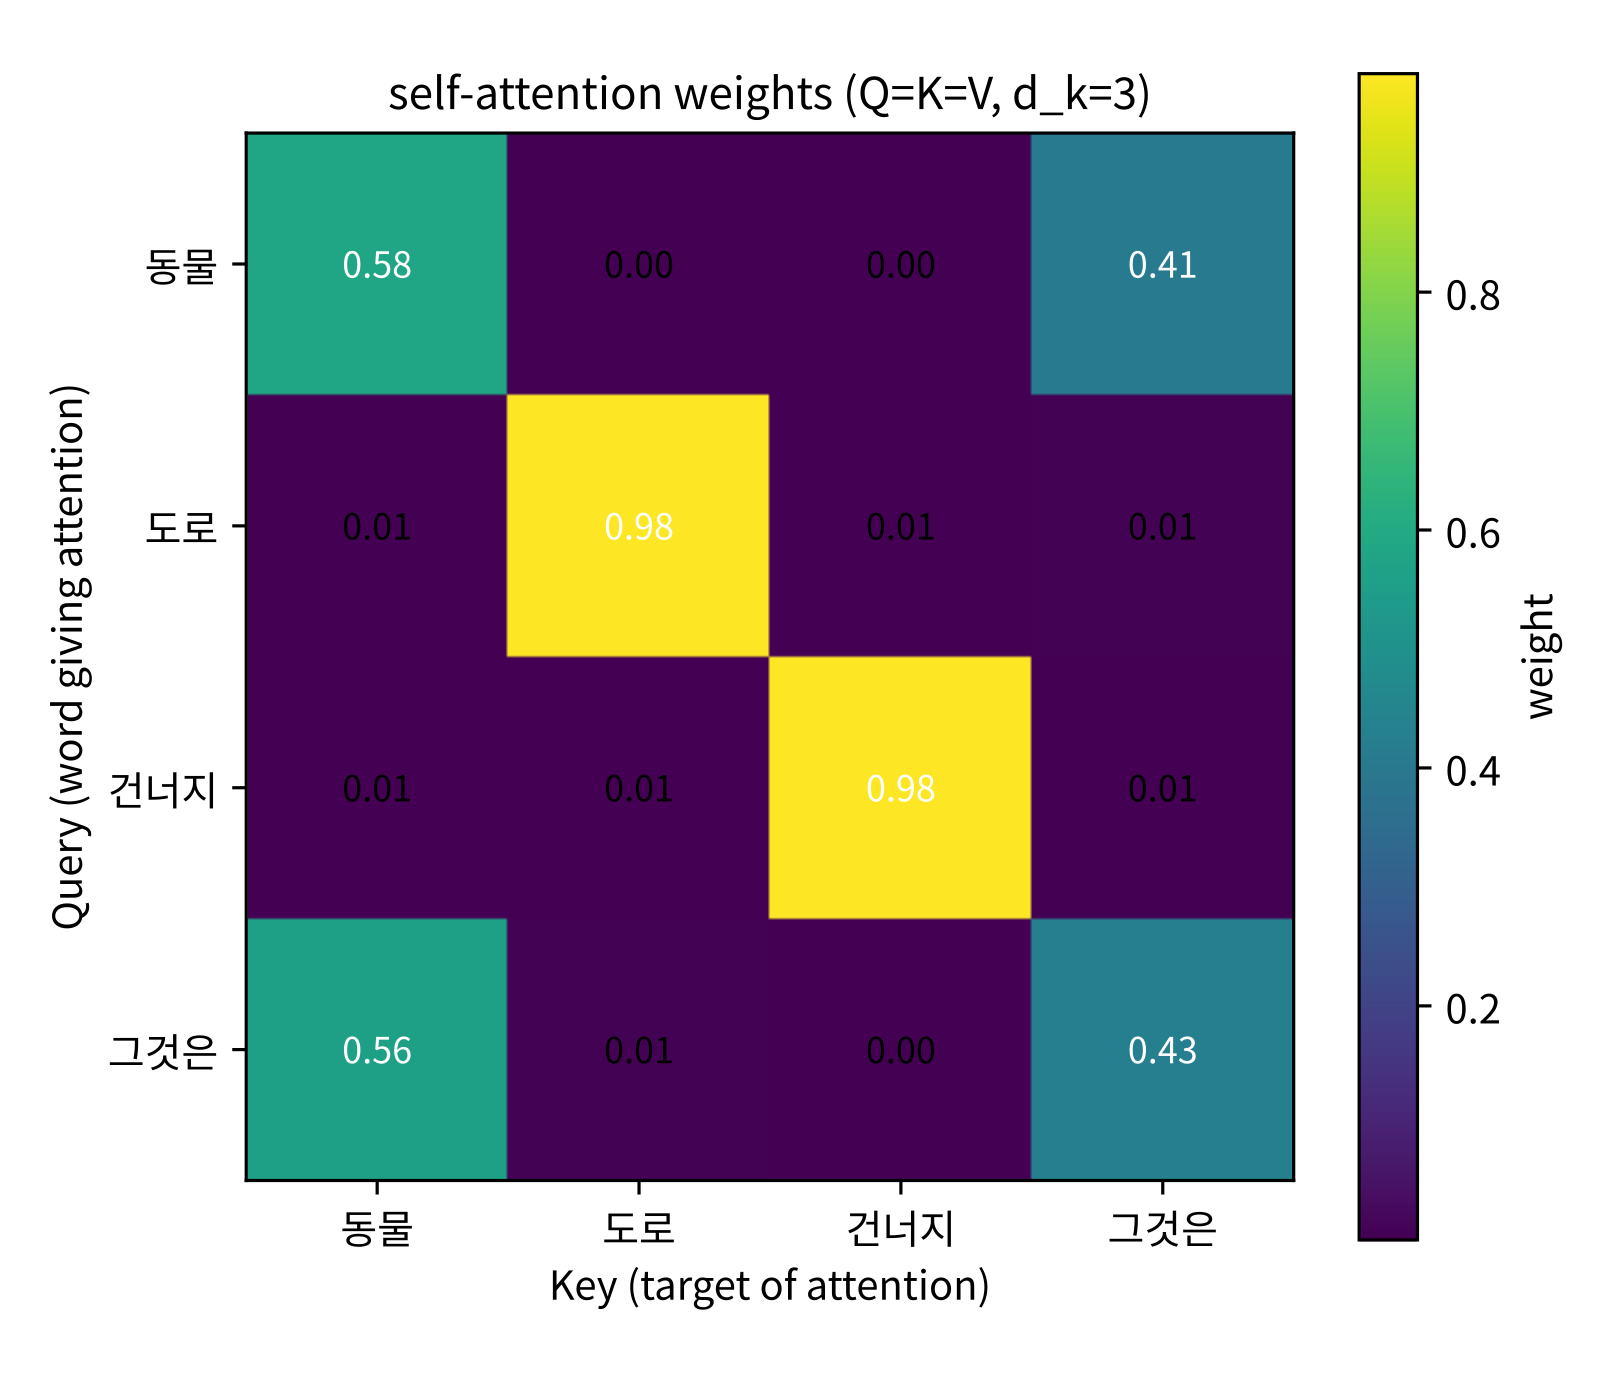
\includegraphics[width=\linewidth]{ch12_2_attention_heatmap.png}
    \end{column}
  \end{columns}
  {\footnotesize ``그것은'' 행이 ``동물'' 열(0.561)과 자기 자신
  열(0.427)에만 높은 값 — 대명사-선행사 관계가 숫자로 구현된
  모습. 나머지 행은 대각선(자기 자신)에 집중.}
\end{frame}

\begin{frame}{왜 softmax가 이렇게 극단적인가 — 원점수에서}
  ``같은 계산을 \textbf{원점수 단계}에서 한 번 더 펼쳐보면'' 왜
  softmax가 이렇게 극단적인 가중치를 내는지 선명해진다:
  \begin{itemize}
    \item $QK^T/\sqrt{3}$ 의 ``그것은'' 행은
      \textbf{$[4.85,\ 0.52,\ 0.0,\ 4.578]$} — ``동물''(4.85)과
      자기 자신(4.578)이 다른 두 단어(0.52, 0.0)보다 \emph{크게}
      벌어져 있다.
    \item softmax가 이 \textbf{4.85 vs 0.52의 차이를 지수적으로
      증폭} ($\approx e^{4.33} \approx 75$배)해서
      \textbf{56\% vs 0.7\%}의 가중치로 변환.
  \end{itemize}
  \vskip0.4em
  \begin{block}{두 단계의 ``스케일이 다르다''}
    softmax \emph{이전}: ``동물''과 ``도로''의 원점수 차이
    \textbf{4.33}이라는 \emph{절대적 크기}.
    softmax \emph{이후}: \textbf{56배의 가중치 비}라는
    \emph{상대적 비율}.
    --- 이 스케일 차이가 ``softmax가 차이를 증폭한다''는
    관찰의 \emph{구체적 수치}다.
  \end{block}
\end{frame}

\begin{frame}{이 예의 한계를 정확히 짚어두기}
  \begin{itemize}
    \item 위 계산은 \textbf{임베딩을 손으로 설계}한 것 —
      ``그것은이 동물과 관련 있다''는 \emph{설계}가 결과에 그대로
      담기는 \textbf{``확인 실험''(confirmation experiment)}에
      가깝다. 실제 모델에서는 이 임베딩과 $W_Q, W_K, W_V$ 가
      \emph{데이터로부터 학습}되어 ``의미적으로 관련된 단어가
      서로 높은 원점수를 낸다''는 패턴이 \emph{스스로}
      만들어진다.
    \item 이 예의 $d_k = 3$ 은 너무 작아 $\sqrt{d_k}$ 스케일링의
      ``극단화 방지'' 효과가 실제로는 \emph{약하게} 보인다
      (원점수가 0$\sim$5 범위라 softmax가 이미 충분히
      분화되어 있음).
    \item $d_k$ 가 크면(예: 512) 원점수가
      $\sqrt{d_k} \approx 23$ 스케일로 벌어져 \textbf{스케일링이
      없으면 one-hot으로 붙는 것} — 앞 절의 ``무작위 내적
      분산'' 논리의 \textbf{본 장면}.
  \end{itemize}
\end{frame}

\begin{frame}{자주 하는 실수: $QK^T$ 의 행/열 방향 혼동}
  $QK^T$ 가 $n \times n$ 행렬인 것은 알지만, \textbf{$(i, j)$
  성분이 ``$i$번째 Query가 $j$번째 Key와 관련 있는 점수''인지
  그 반대인지}를 헷갈리는 것이 이 절의 \textbf{가장 흔한 실수}.
  \vskip0.4em
  확인법은 단순: $QK^T$ 의 $(i,j)$ 성분은 $Q$ 의 $i$번째 \emph{행}과
  $K^T$ 의 $j$번째 \emph{열}, 즉 $Q$ 의 $i$번째 행과
  \textbf{$K$ 의 $j$번째 \emph{행}}의 내적.
  \vskip0.4em
  \begin{block}{읽는 법}
    \textbf{행} = ``\emph{어떤} 단어가 (Query로) \emph{보고
    있는가}'' (누가 주의를 \emph{주고} 있나) \\
    \textbf{열} = ``\emph{어떤} 단어가 (Key로) \emph{보고받고
    있는가}'' (누가 주의의 \emph{대상}인가)
  \end{block}
  네 단어 예에서: ``그것은''의 \emph{행}(4번째,
  $[0.561, 0.007, 0.004, 0.427]$) = ``그것은이 \emph{각
  단어에} 주는 주의''. ``동물''의 \emph{열}(1번째,
  $[0.582, 0.005, 0.005, 0.561]^T$) = ``\emph{각 단어가}
  '동물'에 주는 주의''.
\end{frame}

\begin{frame}{어텐션은 대칭적이지 않다}
  \begin{itemize}
    \item ``그것은 $\to$ 동물''의 가중치 \textbf{0.561}은
      ``동물 $\to$ 그것은''의 가중치 \textbf{0.412}와
      \emph{같지 않다}.
    \item \textbf{어텐션은 \emph{대칭적이지 않다}.}
    \item 이유: $QK^T$ 가 $KQ^T$ 와 일반적으로 다르다 —
      \emph{내적}은 \emph{대칭}이지만, $Q$ 와 $K$ 가
      \emph{서로 다른} 변환 $W_Q, W_K$ 를 거치므로
      ``내가 찾는 것''과 ``내가 가진 것''이 서로 다를 수
      있다.
    \item 12.1절 FAQ에서 ``왜 Q, K, V를 나눕는가''의 정답이
      바로 이 \textbf{비대칭}에서 온다.
  \end{itemize}
  \vskip0.5em
  실습에서는 \textbf{어텐션 행렬을 시각화}해서 확인:
  ``\emph{행} = Query, \emph{열} = Key''라 적힌 라벨을 보고,
  ``그것은''의 \emph{행}이 ``동물'' \emph{열}과 만나는 칸
  (= 0.561)이 ``그것은이 동물에 주는 주의''임을 직접 확인.
  이 ``어떤 칸을 읽고 있는지''를 직관적으로 잡는 것이,
  12.3절 멀티헤드에서 ``\textbf{각 헤드가 어떤 관계를 포착하는가}''를
  읽는 기초가 된다.
\end{frame}

\begin{frame}{자주 하는 실수: $d_k$ 를 ``임베딩 차원''으로 오해}
  \kq{$\sqrt{d_k}$ 의 $d_k$ 가 ``임베딩 차원''이라는 것은
  \emph{아니다}.}
  \begin{itemize}
    \item $d_k$ 는 \textbf{Key 벡터의 차원}, 즉 $W_K$ 가
      \emph{만들어낸} 벡터의 길이.
    \item 12.1절에서 $K = XW_K$ 로, $W_K$ 가 입력 임베딩 차원
      $d_{model}$ 에서 \textbf{$d_k$ 차원으로 \emph{투영}}하는
      변환임을 보았다.
    \item $d_{model} = 512$ 인데 $d_k = 64$ 라면, $K$ 는 64차원
      벡터이고 스케일 상수는 $\sqrt{64} = 8$.
  \end{itemize}
  \vskip0.5em
  이 투영 자체가 \textbf{파라미터 수를 줄이는 효과}(512$\times$512
  행렬 대신 512$\times$64)를 주기도 하지만, \emph{그것보다
  중요한 역할}은:
  \begin{itemize}
    \item \textbf{``비교에 쓸 차원''($d_k$)과 ``전달할 내용의
      차원''($d_v$, Value의 차원)을 \emph{독립적으로} 설계}할 수
      있게 해준다.
  \end{itemize}
  이 ``\textbf{비교 차원 vs 내용 차원을 분리}하는 아이디어''가
  12.3절의 \textbf{멀티헤드 설계}(각 헤드가 \emph{자신의} 작은
  $d_k, d_v$ 를 가짐)의 직접적 전제 조건이 된다.
\end{frame}

\begin{frame}{확인 문제 4개(요약)}
  \begin{enumerate}
    \item \textbf{(원점수 손계산)} $n=3, d_k=2$ 로 $QK^T$ 를
      구하고, 3번째 행을 $\sqrt{2}$ 스케일링 + softmax.
      힌트: $Q$ 의 3번째 행 $(1,1)$ 과 $K$ 의 세 행
      $(1,0),(1,1),(0,1)$ 의 내적 = 1, 2, 1 $\Rightarrow$
      $[0.707, 1.414, 0.707] \to \approx [0.248, 0.503, 0.248]$
      — \emph{가운데 $K$ 에 가장 높은 가중치}.
    \item \textbf{(스케일링의 효과)} 네 단어 예($d_k=3$)의
      임베딩을 10배로 확대하면 $QK^T$ 는 $100$배 $\Rightarrow$
      $\sqrt{d_k}$ 스케일링은 그대로이므로 softmax가 극단적으로
      one-hot. ``스케일링 상수는 \emph{초기} 분산 기준이라,
      임베딩 스케일이 변하면 \emph{다시} 조정''해야 한다.
    \item \textbf{(순서에 대한 대칭)} 임베딩 $[x_1, x_2]$ 와
      순서 뒤집은 $[x_2, x_1]$ 에 self-attention 적용 —
      각 단어의 \emph{출력(대표)}은 같지만, $W$ 행렬은
      \emph{행/열 인덱스가 재배열}된
      \textbf{퍼뮤테이션-등변} 관계. ``순서 정보의 결핍''이
      12.3절 PE의 동기.
    \item \textbf{(볼록성 검증 — 코드)} 각 출력 벡터가 $V$ 의
      4개 원행 \emph{최소/최대 성분 범위} 안에 있는지 필요
      조건으로 확인. (``볼록 껍질 안에 있으면 범위에 반드시
      있지만, 범위에 있어도 볼록 껍질 안에 있지 않다'')
  \end{enumerate}
\end{frame}

\begin{frame}{자주 묻는 질문 1: 문법적으로 ``옳은'' 대상에 집중하나}
  \kq{어텐션 가중치가 항상 ``문법적으로 옳은'' 대상에 집중
  하나요?}
  \begin{itemize}
    \item \textbf{항상 그렇지 않다.} 학습된 모델의 어텐션 헤드를
      실제로 들여다보면, 어떤 헤드는 정확히 대명사-선행사 관계에
      집중하지만, 다른 헤드는 그냥 \textbf{바로 이웃한 단어나
      문장부호}에 집중하는 등 사람이 보기에 ``덜 해석 가능한''
      패턴을 학습하기도 한다 (Michel et al., 2019).
    \item 12.3절의 \textbf{멀티헤드 구조}가 바로 이런
      ``서로 다른 역할을 가진 여러 헤드''를 \emph{병렬로} 두는
      이유.
  \end{itemize}
\end{frame}

\begin{frame}{자주 묻는 질문 2·3: 변환이 없으면?}
  \kq{softmax 없이 내적값을 바로 가중치로 쓰면 안 되나요?}
  내적값은 \textbf{범위가 정해져 있지 않고}(음수 가능), 단어마다
  \textbf{스케일이 달라져} ``합이 1'' 보장이 없으니 출력 스케일이
  불안정. softmax는 Ch.\,2.3 로지스틱회귀와 \textbf{동일한 역할} —
  임의의 실수를 ``\textbf{합이 1인, 항상 양수인} 분포''로 바꿔
  안정적인 \textbf{보간(interpolation)}으로.
  \vskip0.4em
  \kq{$V$ 도 같은 임베딩에서 나오는데, 왜 \emph{서로 다른}
  $W_V$ 가 필요한가? $V = X$ 로 못 하나?}
  \begin{itemize}
    \item 가능하지만 \textbf{표현력이 제한}: $V = X$ 라면 출력은
      ``입력 임베딩들의 가중합''이므로 \textbf{한 층의 출력이 항상
      \emph{입력 임베딩 공간} 안에 갇혀} 있다.
    \item $W_V$ 를 두면 ``\textbf{비교에 쓰는 표현}(Q,K)''과
      ``\textbf{전달하는 내용}(V)''을 \emph{서로 독립적으로}
      학습 — 예: ``그것은''의 \emph{Key}는 ``나를 가리킬 명사''에
      높은 점수를 줘야 하고(비교용), \emph{Value}는 ``지쳐 있음''
      같은 \emph{내용}을 담아줘야 — 두 \emph{역할}을 \emph{같은}
      벡터로 동시에 충당하기 어렵다.
  \end{itemize}
  {\footnotesize 참고: ``$Q=K=V=X$''만으로도 \emph{어텐션
  가중치} 자체는 \emph{일단} 계산된다 (앞 실습이 그 설정) —
  가중치 패턴이 \emph{의미적으로 잘} 나오는지는 $W_Q, W_K, W_V$ 가
  \emph{학습}되었을 때의 문제.}
\end{frame}

\begin{frame}{자주 묻는 질문 4: softmax의 그래디언트}
  $p_i = e^{s_i} / \sum_j e^{s_j}$ 의 $s_k$ 에 대한 미분:
  \[\frac{\partial p_i}{\partial s_k}
    = p_i(\delta_{ik} - p_k)
    \qquad (\text{크로네커 델타 } \delta_{ik})\]
  해석: ``내 확률 $p_i$ 가, \emph{내} 원점수 $s_k$ 를 \emph{올리면}
  $p_i(1 - p_k)$ 만큼 \emph{증가}하고, \emph{다른} 원점수
  $s_j\,(j \neq k)$ 를 올리면 $p_i p_j$ 만큼 \emph{감소}.''
  \vskip0.5em
  \begin{block}{중요한 관찰}
    \textbf{$p_i$ 가 1에 가까우면(one-hot)} $1 - p_k
    \approx 1 - p_i \approx 0$ 이 되어 그 방향의
    \textbf{그래디언트가 사실상 0} — ``이미 한 단어를 독점하면,
    그 선택을 바꿀 학습 신호가 거의 안 온다.''
    이게 ``softmax가 one-hot으로 붙으면 \emph{학습이
    멈춘다}''는 앞 절 관찰의 \textbf{정확한 미분적 근거}.
  \end{block}
  {\footnotesize 이 미분 공식 자체는 Ch.\,3 다중 분류 교차엔트로피
  그래디언트 $(p - y)$ 와 \emph{정확히 같은} 구조 —
  ``softmax + 교차엔트로피''의 그래디언트가 \emph{선형}으로
  단순해지는 이유를 Ch.\,3에서 본 바로 그 사실.}
\end{frame}

\begin{frame}{자주 묻는 질문 5: ``자기 주입''은 왜 대각선이
  높나}
  Q와 K가 \emph{같은} 임베딩이면,
  $q_i \cdot k_i = \|q_i\|^2 \ge 0$ (자기 자신과의 내적 =
  \textbf{노름 제곱, 항상 0 이상}).
  \vskip0.4em
  \textbf{Cauchy-Schwarz} 부등식 $q_i \cdot q_j
  \le \|q_i\|\,\|q_j\|$ 에 따르면, 다른 단어와의 내적이
  \emph{자기 자신과의 내적보다} 클 수 있는 경우는 $q_j$ 의
  노름이 $q_i$ 보다 \emph{크고} 방향까지 \emph{비슷}할 때뿐 —
  임베딩 노름이 서로 비슷하면 \textbf{자기 자신과의 내적이
  \emph{최대}가 되는 구조}.
  \vskip0.4em
  네 단어 예에서 ``도로''가 자기 자신에 \textbf{98.0\%}를 주는
  것이 정확히 이 구조의 산출물 — ``도로''와 \emph{다른} 단어
  (동물 $(3,0,0)$, 건너지 $(0,0,3)$)와의 내적이 0인 반면,
  ``도로''와 \emph{자기 자신} $(0,3,0)$ 과의 내적이
  $3^2 = 9$ 이어서 softmax에서 압도적.
  \vskip0.3em
  이 ``자기 주입''은 \textbf{\emph{단점}이 \emph{아니다}} —
  각 단어의 표현에 \emph{자기 자신의} Value를 \emph{기본적으로}
  포함시켜 ``이 단어의 \emph{기존} 정보가 \emph{완전히} 사라지지
  않고'' \emph{다른} 단어의 정보가 \emph{추가}되는 형태''로
  동작 → \textbf{학습 안정성에 긍정적}.
  \vskip0.3em
  {\footnotesize ``자기 주입 + 잔차'' 조합은 10.2절 ResNet(He et
  al., 2015)의 $y = F(x) + x$ 와 \emph{정신적으로} 닮아 있다 —
  ``출력 = 입력의 일부 + 새로운 정보'' 패턴.}
\end{frame}

% ===== SECTION 12.3 =====
\section{12.3 멀티헤드 어텐션과 포지셔널 인코딩}
\begin{frame}{Multi-Head Attention: 관점을 병렬로}
  Q, K, V를 한 세트만 쓰는 대신, \textbf{여러 세트(``헤드'', head)}를
  병렬로 두고 각각 \textbf{다른 관점}의 관련성을 학습하게 한다
  (Vaswani et al., 2017):
  \begin{itemize}
    \item 한 헤드는 \textbf{문법적 관계}(주어-동사)에, 다른 헤드는
      \textbf{의미적 관계}(동의어)에 집중하는 식으로 역할이 나뉘는
      경향이 관찰된다.
    \item 여러 헤드의 결과를 \textbf{이어붙인(concatenate)} 뒤
      다시 한 번 \textbf{선형변환}해서 최종 출력을 만든다.
  \end{itemize}
  \vskip0.5em
  \begin{block}{Ch.\,7.2 랜덤 포레스트(Breiman, 2001)와 같은 직관}
    ``서로 다른 트리 여러 개의 다수결''로 단일 트리보다 안정적인
    예측을 얻었던 것과 비슷. 다만 RF의 트리들은 \textbf{무작위성}만으로
    다양해지는 반면, 멀티헤드의 각 헤드는 \textbf{역전파}를 통해
    ``서로 다른 역할을 맡는 것이 전체 손실을 줄이는 데 유리하다''는
    방향으로 \textbf{스스로 분화}한다는 차이가 있다.
  \end{block}
\end{frame}

\begin{frame}{왜 헤드 하나가 부족할까 — ``관점''의 문제}
  \kq{``크기''의 문제가 아니라 \textbf{``관점''}의 문제.}
  \begin{itemize}
    \item 한 개의 어텐션 헤드는 단어 쌍마다 \textbf{점수(내적)
      하나}를 만든다 — 그 하나의 숫자가 그 쌍의 \emph{모든}
      관계를 짊어져야 한다.
    \item 실제 언어에서 ``단어 $i$와 $j$가 얼마나 관련 있는가''는
      \textbf{여러 독립적 요인의 합}: 문법(주어-동사, 대명사-선행사),
      의미(동의어, 상위어), 위치(바로 앞의 단어), 문장부호 등.
    \item 두 요인이 \textbf{거의 반대 방향}으로 작용하는 쌍이 항상
      존재: ``그것은''은 문법적으로는 ``동물''을 봐야 하지만
      (선행사), ``도로''와 문맥상 더 가깝게 쓰일 수도 있다
      (의미).
    \item 한 개의 점수는 이 둘을 \textbf{타협}해야 하지만, 두 개의
      헤드는 각자 하나의 요인에 \emph{전부} 집중할 수 있다 —
      헤드가 두 개라 \textbf{``타협 대신 전담''}이 가능.
  \end{itemize}
\end{frame}

\begin{frame}{기하학적으로: 볼록 결합에서 직합으로}
  12.2절의 볼록성 논리를 떠올리면:
  \begin{itemize}
    \item 한 헤드는 각 단어에 대해 $V$ 원행들의 \textbf{볼록
      결합 하나}(볼록 껍질 안의 점 하나)를 만든다.
    \item 한 개의 헤드로는 각 단어에 ``\textbf{하나의} 혼합
      비율''만 표현되지만, $h$개의 헤드는 ``$V_1$·$V_2$를 이
      비율로 섞은 것''과 ``$V_3$·$V_4$를 저 비율로 섞은 것''을
      \textbf{서로 독립적으로} 표현할 수 있다.
    \item 표현 가능한 영역이 \textbf{단일 볼록 결합에서 여러
      부분공간의 볼록 결합의 \emph{직합(direct sum)}으로 넓어진다}.
  \end{itemize}
  \vskip0.5em
  \begin{block}{랜덤 포레스트 비유를 다시}
    단일 트리가 ``한 번의 투표''라면 포레스트는 \emph{여러 투표의
    병합}. 헤드들도 마찬가지로 \textbf{``한 관점의 투표를 여러
    개 붙여 놓는''} 것이다.
  \end{block}
\end{frame}

\begin{frame}{멀티헤드 공식}
  모델 차원 $d_{model}$ 을 $h$개의 헤드에 나눠, $i$번째 헤드는
  $d_k = d_{model}/h$ 차원의 Q, K, V 위에서 12.2절의 어텐션을
  계산:
  \[
  \text{MultiHead}(Q,K,V) =
  \text{Concat}(\text{head}_1, \dots, \text{head}_h)\, W_O,
  \qquad
  \text{head}_i = \text{Attention}\!\left(QW_i^Q,\; KW_i^K,\;
  VW_i^V\right)
  \]
  \begin{itemize}
    \item $W_i^Q, W_i^K \in \mathbb{R}^{d_{model} \times d_k}$,
      $W_i^V \in \mathbb{R}^{d_{model} \times d_v}$:
      \textbf{헤드별 투영 행렬} — 각 헤드가 ``무엇과 무엇을
      비교할지''(Q·K)와 ``무엇을 전달할지''(V)를 \emph{각자}
      학습(12.1절의 Q/K/V 삼분 구조가 \textbf{헤드마다 하나씩}).
    \item $W_O \in \mathbb{R}^{h d_v \times d_{model}}$:
      이어붙인 결과를 다시 $d_{model}$ 차원으로 — ``각 헤드의
      정보를 어떻게 섞어 다음 층에 줄지''를 결정하는
      \textbf{최종 선형변환}.
  \end{itemize}
\end{frame}

\begin{frame}{$d_{model}$ 을 $h$로 나눈 이유}
  \kq{헤드를 ``크게'' 만드는 것이 아니라 \textbf{``다'' 만드는
  것}.}
  \begin{itemize}
    \item 헤드 수를 늘리되 헤드당 차원을 줄이지 않으면(각
      헤드도 $d_{model}$ 차원 그대로), QKV 파라미터가 \textbf{헤드
      수만큼 \emph{배}로} 늘어난다.
    \item $d_k = d_{model}/h$ 로 나눠야 \textbf{파라미터 수가
      \emph{단일 헤드와 (거의) 같다}}:
  \end{itemize}
  \[
  \underbrace{h \times 3 \times d_{model} \times
    \frac{d_{model}}{h}}_{\text{h 헤드의 QKV 합계}}
  = 3\, d_{model}^2
  \;=\;
  \underbrace{3 \times d_{model} \times d_{model}}_{\text{단일
  헤드 QKV}}
  \]
  \vskip0.3em
  $d_{model}=512,\; h=8$ 으로 대면: $8 \times 3 \times 512
  \times 64 = 786{,}432 = 3 \times 512 \times 512$ —
  \textbf{정확히 같다}. (여기에 $W_O$(512$\times$512 =
  262,144)만 더해진다.)
  \vskip0.3em
  \begin{block}{설계의 요지}
    \textbf{파라미터 비용을 거의 그대로 유지한 채 독립적 관점의
    수를 $h$배로 사는} 것 — 더 많은 파라미터가 아니라
    \emph{같은} 파라미터를 \textbf{재배분}하는 설계.
    (12.2절 ``$d_k$ 는 임베딩 차원이 아니라 \emph{헤드당} Key
    차원''이라는 사실의 설계적 귀결.)
  \end{block}
\end{frame}

\begin{frame}{손으로 한 번: 두 헤드(자기 / 이웃)}
  단어 2개(임베딩 $x_1=(1,0),\; x_2=(0,1)$) 예에서 두 헤드를
  직접 설계:
  \begin{itemize}
    \item \textbf{헤드 A} (자기): $W_Q = W_K = W_V = I$ —
      12.2절의 ``자기 주입'' 헤드.
    \item \textbf{헤드 B} (이웃): 그것과 \textbf{$W_K$ 하나만}
      $\begin{pmatrix}0&1\\1&0\end{pmatrix}$ (두 차원을 바꾸는
      행렬)로 달라도, $Q=K=V=X$ 에서 $K$ 만 이 행렬을 거치면
      각 단어가 \emph{다른} 단어의 Key와 더 잘 맞게 되어
      ``이웃 우선'' 헤드.
  \end{itemize}
  \small
  \begin{tabular}{@{}lllp{6cm}@{}}
    \toprule
    헤드 & $W_K$ & 어텐션 가중치 (행=Query) & 읽기 \\
    \midrule
    A (자기) & $I$ & (0.670, 0.330) / (0.330, 0.670) &
      각 단어가 \textbf{자기 자신}에 67\% \\
    B (이웃) & $\begin{pmatrix}0&1\\1&0\end{pmatrix}$ &
      (0.330, 0.670) / (0.670, 0.330) &
      각 단어가 \textbf{다른 단어}에 67\% \\
    \bottomrule
  \end{tabular}
  \vskip0.5em
  두 행렬은 \textbf{완전한 미러}다 — A 헤드의 ``자기 우위''
  방향이 바로 B 헤드의 ``이웃 우위'' 방향. $V$ 가 같은데도
  \textbf{출력이 다르다}:
  \begin{itemize}
    \item 헤드 A의 단어 1 출력 = $[0.670, 0.330]$
    \item 헤드 B의 단어 1 출력 = $[0.330, 0.670]$
  \end{itemize}
  {\footnotesize 가중치가 반대라 섞임 비율이 뒤집힌 것.}
\end{frame}

\begin{frame}{이어붙임: 하나의 벡터 안에 두 관점}
  $W_O = I_4$ (연결만 하고 더 이상 섞지 않는 가장 단순한 경우)로
  이어붙이면, 단어 1의 4차원 출력은
  \[ [0.670,\; 0.330,\; 0.330,\; 0.670], \qquad
     \text{단어 2: } [0.330,\; 0.670,\; 0.670,\; 0.330] \]
  읽어보면: 앞 2차원(헤드 A) = ``단어 1의 자기는 $V_1$, 단어 2의
  자기는 $V_2$'' 라는 사실; 뒤 2차원(헤드 B) = ``단어 1의 이웃은
  $V_2$, 단어 2의 이웃은 $V_1$'' 라는 \textbf{다른} 사실.
  단일 헤드의 2차원 출력은 이 두 사실 중 \textbf{하나만} 담을 수
  있었는데, \textbf{멀티헤드는 두 사실을 \emph{같은 벡터 안의
  서로 다른 부분공간}에 나란히 넣었다}.
  \vskip0.3em
  {\footnotesize 실제 학습에서는 ``자기/이웃 헤드''를 누가 맡을지
  \textbf{사람이 설계하지 않는다} — 손실이 줄어드는 방향으로
  역전파가 각 헤드의 $W_i^Q, W_i^K, W_i^V$ 를 \emph{스스로} 다른
  역할로 벌려놓는다.}
  \vskip0.3em
  \kq{그런데 왜 ``합치기(평균/합산)''가 아니라 ``이어붙이기''인가?}
  합하면 $h$개 헤드의 정보가 다시 하나의 벡터로 \textbf{재혼합}되어
  각 헤드의 독립적 관점이 \textbf{희석}된다 — 미러 예에서 숫자로
  확인: 두 헤드 출력을 \emph{더하면}
  \[ [0.670,0.330] + [0.330,0.670] = [1.0, 1.0] \quad
     (\text{단어 2도 } [1.0, 1.0]) \]
  \textbf{두 단어의 출력이 정확히 \emph{같아진다}!} — 미러였던 두
  관점이 합산되는 순간 ``이 단어와 저 단어가 다르다''는 정보가
  \emph{소거}된다. 이어붙임은 각 헤드 출력을 \textbf{서로 다른
  차원(부분공간)}에 두어 소거를 \emph{막고}, $W_O$ 가 ``출력
  차원 $j$는 $i$번째 헤드의 몇번째 성분을 얼마 신뢰할지''를
  결정하게 한다 — ``\textbf{관점의 조합}''을 다음 층(피드 포워드)이
  결정하도록 \textbf{자유도를 남겨둔다}.
  {\footnotesize 실제 학습된 $W_O$ 는 대각선 근방의 ``출력 차원 $j$
  $\leftarrow$ 헤드 $i$의 $k$번째 성분'' 같은 \textbf{희소 패턴}이
  자주 관찰된다.}
\end{frame}

\begin{frame}{세 단어 [개, 고양이, 쫓는다]: 서로 다른 3개 헤드}
  \begin{columns}[T]
    \begin{column}{0.55\textwidth}
      \begin{itemize}
        \item \textbf{(a) 자기-우위 헤드}: $Q=K=V$ 로
          self-attention — 12.2절 ``자기 주입'' 효과
          (자기 자신과의 내적 $\|q_i\|^2$ 가 최대)로
          \textbf{대각선 우세} (``개'' 0.78, ``고양이'' 0.74,
          ``쫓는다'' 0.93).
        \item \textbf{(b) 위치-유사 헤드}: \emph{Key만}
          1위치 순환 이동 ($K_i = E_{i+1}$) — 각 단어는
          \textbf{다음 단어}의 Key와 가장 잘 맞아
          (개$\to$고양이 0.78, 고양이$\to$쫓는다 0.74,
          쫓는다$\to$개 0.93) — \emph{위상(순서)} 정보가
          가중치에 새겨진다.
        \item \textbf{(c) 역할 없음}: 모든 Key를 $(1,1)$ 으로 —
          모든 가중치가 \textbf{0.333 균일}, ``아직 아무
          역할도 분화하지 못한'' 헤드.
      \end{itemize}
    \end{column}
    \begin{column}{0.41\textwidth}
      \centering
      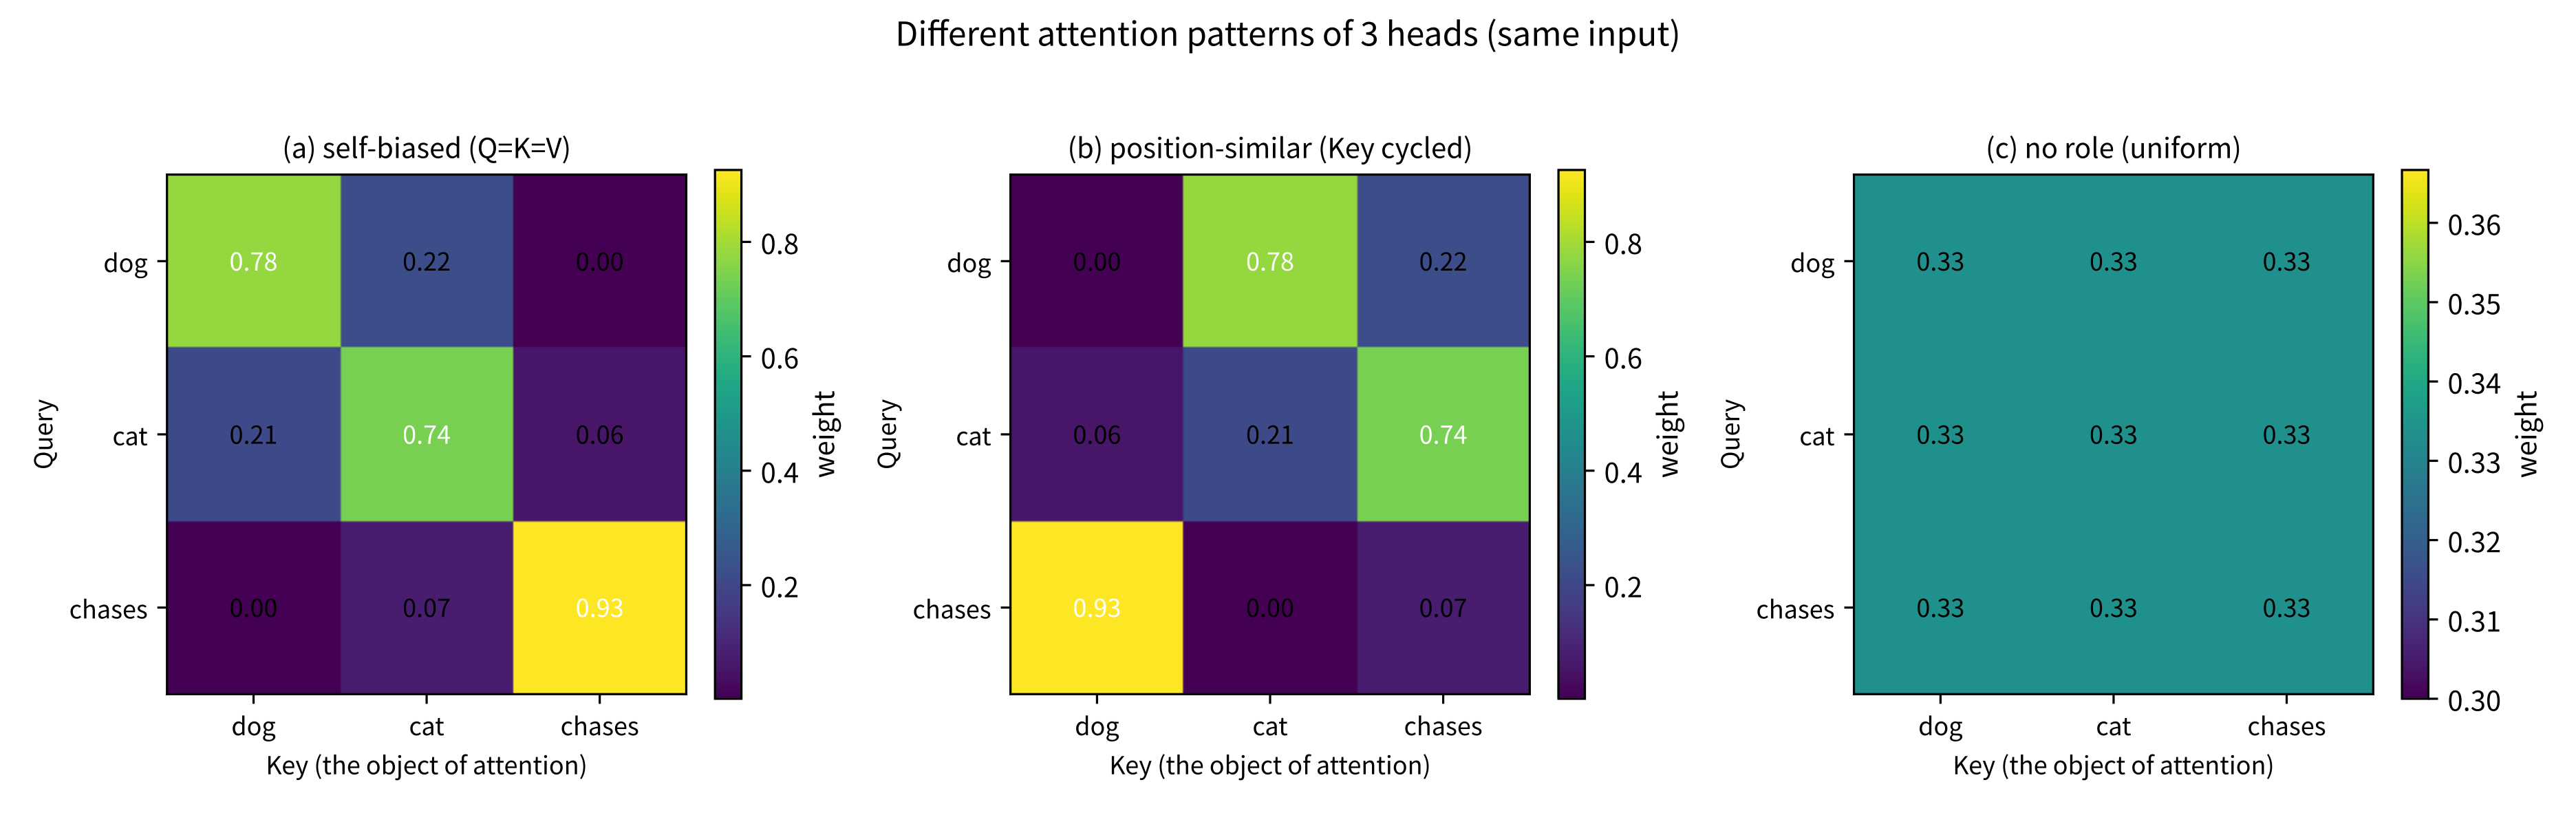
\includegraphics[width=\linewidth]{ch12_3_multihead_weights.png}
      \vskip0.2em
      {\footnotesize 3단어에 대해 패턴이 서로 다른 3개 헤드.
      학습된 모델에는 (a)(b) 같은 서로 다른 패턴의 헤드들이
      실제로 공존한다.}
    \end{column}
  \end{columns}
\end{frame}

\begin{frame}{역사: 헤드 역할 분화는 관측된 사실인가}
  \begin{columns}[T]
    \begin{column}{0.56\textwidth}
      \textbf{네} — ``인터프리테이빌리티'' 연구로 실제로 확인:
      \begin{itemize}
        \item Clark·Khandelwal·Levy·Manning (``What does BERT
          look at?'', 2019)은 BERT(Devlin et al., 2018)의 헤드를
          하나씩 분석:
          \begin{enumerate}
            \item \textbf{바로 앞 단어만} 보는 ``위치 헤드''
            \item \textbf{같은 품사}의 단어끼리 집중하는 헤드
            \item \textbf{문법적 통사}(주어-구문)를 추적하는 헤드
          \end{enumerate}
          가 \textbf{분명히 존재}함을 보였다.
        \item \textbf{부수적 결과}: 헤드의 50$\sim$60\%를
          \emph{임의}로 제거해도 성능 저하 \textbf{매우 작다} —
          역할 분화는 실제로 있으면서도 \textbf{여분(redundancy)}이
          크다 (이 때문에 \textbf{헤드 프루닝} (Michel et al.,
          2019)이 추론 속도 기법으로 쓰임).
        \item \textbf{주의}: \emph{어떤} 헤드가 \emph{어떤}
          역할을 맡는가는 학습 run마다 \textbf{다르다}.
      \end{itemize}
      \vskip0.3em
      {\footnotesize 2017년 ablation: 헤드를 8$\to$\textbf{1개}로
      줄이면 BLEU가 \textbf{약 1점} 감소 (EN-DE 24.16$\to$23.48,
      EN-FR 38.19$\to$37.19) — ``관점 하나만''이면 눈에 띄게
      손해; 8개 이상은 \textbf{감소수익}. 헤드당 차원이 너무
      얇아지면($d_k = d_{model}/h$, 예: $h=32$이면 $d_k=16$)
      이득이 사라진다.}
    \end{column}
    \begin{column}{0.4\textwidth}
      \centering
      
\includegraphics[width=\linewidth]{ref_bertbert.png}
      \vskip0.2em
      {\footnotesize ``What Does BERT Look At?'' Figure 5 —
      특정 헤드들은 인접 토큰, 품사 같은 토큰, 통사 구조적으로
      연결된 토큰(주어-동사, 대명사-선행사)에 집중.}
    \end{column}
  \end{columns}
  \vskip0.4em
  \begin{block}{현재 대형 LLM(GPT(Radford et al., 2018),
      LLaMA(Touvron et al., 2023) 등)}
    헤드를 \textbf{수십$\sim$100개 이상} 쓰지만 $d_{model}$ 이
    4096$\sim$8192로 \emph{비례}로 커진 덕분이며,
    \textbf{헤드당 차원은 여전히 64$\sim$128 부근} —
    \textbf{2017년 설계가 그대로 살아 있는 값}.
  \end{block}
\end{frame}

\begin{frame}{Positional Encoding: 순서 정보는 어떻게 넣나}
  어텐션 연산 자체는 \textbf{순서를 전혀 구분하지 않는다} —
  $QK^T$ 는 순서를 뒤섞어도 각 쌍의 관련도 자체는 똑같이
  계산(집합처럼 취급). 그런데 ``강아지가 고양이를 쫓는다''에서는
  \textbf{순서가 의미를 바꾼다}. 그래서 Transformer는 각 단어의
  임베딩에 위치 정보를 담은 벡터(positional encoding,
  \textbf{사인/코사인} 함수의 고정 패턴)를 \textbf{더해서}
  넣는다 — 같은 단어라도 \textbf{위치가 다르면 입력 벡터 자체가
  달라지}므로, 어텐션이 \textbf{간접적으로} 순서를 활용할 수
  있다.
  \vskip0.4em
  ``어텐션은 순서를 구분 못 한다''는 단순한 직관이 아니라,
  \textbf{코드로 확인할 수 있는 정리}:
  \begin{itemize}
    \item 단어 3개 $[\text{개}, \text{고양이}, \text{쫓는다}]$
      (임베딩 $(1,0), (0,1), (2,0)$)와 앞 두 단어를 바꾼
      $[\text{고양이}, \text{개}, \text{쫓는다}]$ 에 PE 없이
      self-attention($Q=K=V$) 적용.
    \item 두 문장의 어텐션 가중치 행렬:
      \[ W_{\text{B}} = P\, W_{\text{A}}\, P^T \]
      (완전히 같은 관계 — $P$ 는 1·2행을 바꾼
      \textbf{퍼뮤테이션 행렬}).
    \item 각 단어의 출력도 \textbf{정확히 퍼뮤테이션}: 문장 A에서
      ``고양이''의 출력 $[0.745,\; 0.503]$ , 문장 B에서
      ``고양이''의 출력도 \textbf{$[0.745,\; 0.503]$} —
      \emph{같은 단어의 표현이 위치에 무관하게 정확히
      같}다. ``누가 누구를 쫓는지''는 \textbf{통째로
      사라졌다}.
  \end{itemize}
  \vskip0.3em
  \begin{block}{permutation-equivariant(퍼뮤테이션-등변)}
    자기 어텐션 전체 연산이 \textbf{입력을 재배열하면 출력도
    같은 방식으로 재배열}. 순서 정보를 \emph{어딘가}에 덧붙여
    주지 않는 한 ``개가 고양이를 쫓는다''와 ``고양이가 개를
    쫓는다''를 구분하는 것은 \textbf{수학적으로 불가능}.
  \end{block}
\end{frame}

\begin{frame}{PE의 수식: 시계 쌍}
  위치 $t$ 의 $d_{model}$ 차원 벡터를, \textbf{짝수 차원에
  사인·홀수 차원에 코사인}을 두는 식:
  \[ PE_{(t,\,2i)} = \sin\!\left( \frac{t}{10000^{2i/d_{model}}}
     \right), \qquad
     PE_{(t,\,2i+1)} = \cos\!\left( \frac{t}{10000^{2i/d_{model}}}
     \right) \]
  \begin{itemize}
    \item 차원 쌍 $(2i, 2i+1)$ 하나하나가 \textbf{``시계(clock)''}
      하나 — 주파수 $\omega_i = 1/10000^{2i/d_{model}}$ 의
      사인/코사인 파동이 위치 $t$ 를 따라 \emph{tock-tock}하는 것.
    \item 가장 작은 $d_{model}=4$ 로 값을 써보면:
  \end{itemize}
  \small
  \begin{tabular}{@{}ll@{}}
    \toprule
    위치 $t$ & $PE(t)$ (d=4) \\
    \midrule
    0 & (0.000, 1.000, 0.000, 1.000) \\
    1 & (0.841, 0.540, 0.010, 1.000) \\
    2 & (0.909, $-$0.416, 0.020, 0.9998) \\
    10 & ($-$0.544, $-$0.839, 0.0998, 0.995) \\
    \bottomrule
  \end{tabular}
  \vskip0.5em
  1번 시계(앞 짝, $\omega=1$)는 \textbf{빠르게}, 2번 시계
  (뒤 짝, $\omega=0.01$)는 \textbf{아주 천천히} 돈다 —
  첫 행에서 뒤 짝이 $(0,1) \to (0.01,1) \to (0.02, 0.9998)$ 로
  \emph{거의 제자리}인 것과 대조.
  $d_{model}=512$ 이면 \textbf{시계 256개} — 가장 빠른 시계
  주기 약 $2\pi \approx 6.3$, 가장 느린 시계 주기 약 60,000.
  \vskip0.3em
  {\footnotesize 확인 문제 3: $d_{model}=4$ 의 1번 시계
  ($\omega=1$)에서 $PE(3)$ 의 앞 2성분 $(\sin 3, \cos 3)
  \approx (0.141, -0.990)$ 에 $R(1) \approx
  \begin{pmatrix}0.540 & 0.841\\ -0.841 & 0.540\end{pmatrix}$ 를
  곱하면 $PE(4)$ 의 앞 2성분 $(\sin 4, \cos 4) \approx
  (-0.757, -0.654)$ 와 일치 — ``\textbf{1위치 이동 =
  1라디안 회전}''.}
\end{frame}

\begin{frame}{256개의 시계 = 거의 유일한 512차원 패턴}
  \begin{columns}[T]
    \begin{column}{0.52\textwidth}
      \begin{itemize}
        \item 256개의 시계가 \emph{모두를} 합치면,
          \textbf{수만 단어 범위 안의 서로 다른 위치마다 거의
          유일한 512차원 패턴}이 생긴다.
        \item 2017년 모델이 \textbf{512 길이의 문장}을 다룰
          수 있었던 이유이기도 하다.
        \item 빠른 시계(주기 $\approx 6.3$)는 \textbf{이웃
          위치}를 구분, 느린 시계(주기 $\approx 60{,}000$)는
          \textbf{문장 전체의 ``대략 어디쯤''}을 표시.
      \end{itemize}
    \end{column}
    \begin{column}{0.44\textwidth}
      \centering
      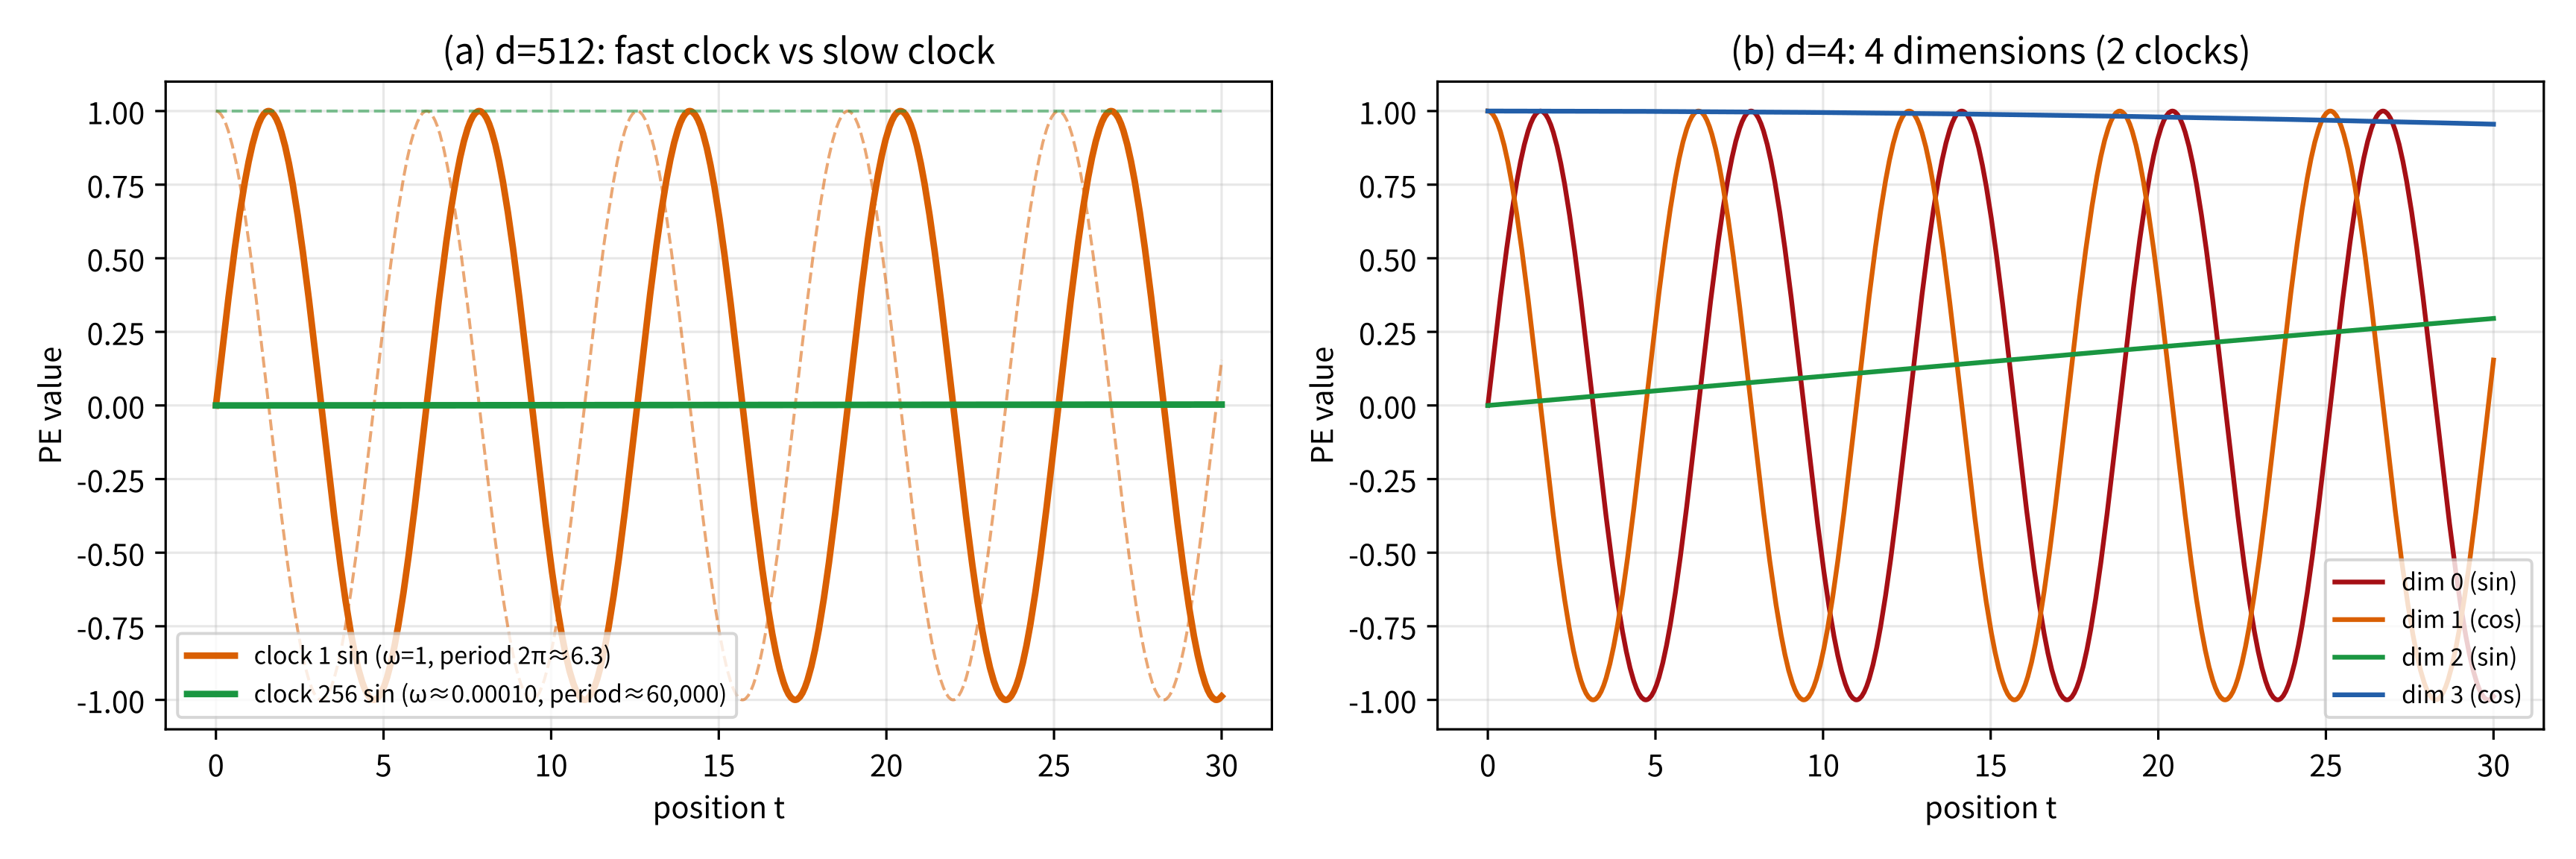
\includegraphics[width=\linewidth]{ch12_3_positional_encoding.png}
      \vskip0.2em
      {\footnotesize (a) d=512의 1번(가장 빠른) 시계 vs 256번
      (가장 느린) 시계의 사인/코사인 곡선. (b) d=4의 4개 차원
      (2개 시계)을 위치 $t=0\sim30$ 에 따라 그린 값 — 서로 다른
      주기의 파동이 겹쳐 \textbf{각 위치마다 고유한 패턴}.}
    \end{column}
  \end{columns}
\end{frame}

\begin{frame}{사인/코사인의 수학: 회전 성질}
  한 시계 쌍을 보면, 위치 $t$ 의 패턴은 \textbf{각도 $t\omega$
  에 있는 ``시계 바늘''}.
  \vskip0.4em
  \kq{핵심 성질: 위치 $k$ 만큼 앞서는 것은, 시계 바늘을
  각도 $k\omega$ 만큼 \emph{돌리는 것}과 \textbf{동일}.}
  \vskip0.4em
  즉, $\omega$ 에만 의존하는 \emph{고정된} 2$\times$2 회전행렬
  $R(\omega)$ 가 존재해
  \[ PE_{(t+k)} = R(\omega)^k \, PE_{(t)} \]
  가 성립(중학 수학의 ``각도 $k$ 회전 = 사인/코사인 가산
  정리의 행렬 버전''). 2시계로 묶어 $R = \text{blockdiag}
  (R(\omega_1), R(\omega_2))$ 로 쓰면, \textbf{$k$개의 위치
  이동은 입력 벡터에 \emph{선형 변환} $R^k$ 를 적용한 것과
  정확히 같}다.
  \vskip0.4em
  \begin{block}{그것이 왜 좋은가 (원논문의 표현)}
    ``각 위치 $t$ 의 PE는 \emph{상대 위치} $k$ 에 대한
    \textbf{선형 함수}로 표현된다'' ($PE_{(t+k)}$ 의 각 성분이
    $PE_{(t)}$ 의 성분들의 선형 결합, 결합 계수는 $k$ 에만
    의존). 즉 \textbf{어텐션의 선형 도구}(Q·K 내적, $W_O$
    선형변환)만으로 ``\textbf{그 단어가 나보다 $k$칸 뒤}''라는
    \emph{상대} 관계를 읽을 수 있다 — ``절대 위치 7''이 아니라
    \textbf{``그 단어와의 \emph{거리 3}''}이 학습 대상.
    \textbf{차분 성질} $PE_{(t+k)} - PE_{(t)} = (R^k - I)\,
    PE_{(t)}$ 는 절대 위치 $t$ 에 \emph{무관}하고 $k$ 만 담는
    패턴을 만듦 (실습 실험 5, $t=3, k=2$ 수치 확인).
  \end{block}
\end{frame}

\begin{frame}{왜 ``더하기''인가 — 그리고 왜 고정된 함수인가}
  \begin{enumerate}
    \item \textbf{임베딩에 \emph{더하면}} 총 차원이 $d_{model}$
      \textbf{그대로}라, 12.1절 이후의 \textbf{모든 행렬
      크기}($W_Q, W_K, W_V$ 의 크기)와 \textbf{파라미터 예산이
      \emph{변하지 않는다}}. (붙여 넣는 concatenate도 변형으로
      가능하지만 \textbf{차원이 두 배가 되는 비용}이 있다.)
    \item \textbf{학습하지 않고 고정 함수를 쓰는 이유}:
      \begin{itemize}
        \item \textbf{학습된 위치 임베딩}: ``학습 때 본 최대
          위치''가 \textbf{정의의 경계}.
        \item $\sin(t/10000^i)$: \textbf{\emph{아무} $t$ 에도
          \emph{정의}된다}.
      \end{itemize}
  \end{enumerate}
  \vskip0.4em
  원논문(Vaswani et al., 2017)은 \textbf{학습된 위치 임베딩도
  \emph{실제} 시도}해 봤고, 결과 차이는 거의 없었으나
  ``\textbf{더 긴 문장 외삽(extrapolation)} 가능성''을 이유로
  사인/코사인 버전을 택했다고 \emph{명시}.
\end{frame}

\begin{frame}{자주 하는 실수: PE를 빼먹고 어텐션만 쓰기}
  12.2절 실습의 \texttt{attention} 함수를 그대로 문장 두 개 —
  ``\textbf{강아지가 고양이를 쫓는다}''와 ``\textbf{고양이가
  강아지를 쫓는다}'' — 에 적용하면, 같은 세 단어로 이루어져
  있으므로 (PE 없이) \textbf{두 문장에 대해 완전히 동일한
  어텐션 가중치와 출력이 나온다} — ``누가 누구를 쫓는지''가
  \textbf{통째로 사라지는 것}. Ch.\,11.1에서 지적한 ``MLP/CNN에
  단어를 \emph{벡터 집합}으로 넣으면 순서 정보가 사라진다''의
  \textbf{형태만 바뀐 재발}: RNN은 \emph{순차 처리 구조
  자체가} 순서를 암묵적으로 인코딩했지만, 어텐션은 \textbf{병렬
  처리를 얻은 대신} 그 암묵적 순서 정보를 잃었다 — PE로
  \emph{명시적으로} 다시 넣어줘야 한다.
  \vskip0.3em
  \begin{block}{정량화}
    PE를 넣자 같은 문장에서 ``쫓는다''의 가중치 행이
    \textbf{(0.187, 0.045, 0.768) $\to$ (0.013, 0.008, 0.979)}
    로 \emph{달라진다} — \textbf{같은 단어라도 위치에 따라
    어텐션이 달라진다}는 것, 이것이 PE가 \emph{실제로} 하는 일
    (실습 노트북 실험 4).
  \end{block}
\end{frame}

\begin{frame}{보너스: Masked Attention — 디코더는 왜
  ``왼쪽만'' 보는가}
  트랜스포머 전체 구성에 필요한 조각이 하나 더 — 어텐션 점수
  행렬에 \textbf{마스크(mask)}를 하는 것:
  \begin{itemize}
    \item 디코더가 $t$번째 단어를 \emph{만드는} 순간, $(t+1)$번째
      이후(\textbf{``미래''})의 정보를 \emph{보아서는 안 된다}.
    \item 실제 생성(추론) 시점엔 \textbf{미래가 아직 존재하지
      않으므로}, 학습 때만 미래를 보고 훈련하면
      \textbf{학습과 추론이 불일치}한다 (Ch.\,6.1 과적합 문제와
      같은 종류).
    \item \textbf{해법}: softmax \emph{이전}의 원점수 행렬에서,
      \textbf{상삼각(``미래'' 위치)에 $-\infty$} (실제로는
      $-10^9$)를 \emph{더함} — $e^{-10^9} \approx 0$ 이므로
      softmax 후 해당 위치의 가중치가 \textbf{정확히 0}.
  \end{itemize}
  \vskip0.3em
  \begin{block}{causal(인과) 마스크의 효과}
    \textbf{학습은 \emph{모든 위치를 병렬로} 계산하되 각 위치가
    \emph{왼쪽만} 보는 것이 가능}해진다 — \textbf{``학습의
    병렬성''과 ``생성의 순차성''을 하나의 마스크가 통일}.
    Ch.\,17 LLM의 \textbf{자기회귀(autoregressive) 생성}은
    정확히 이 메커니즘 위에 있다(디코더의 self-attention이
    ``masked/causal attention''이라 불리는 이유).
  \end{block}
\end{frame}

\begin{frame}{3단어 예: causal mask 전/후}
  \small
  \begin{tabular}{@{}lll@{}}
    \toprule
    위치 & 마스크 \emph{없}은 가중치 행 &
      마스크 \emph{있}(causal) 가중치 행 \\
    \midrule
    1 (개) & (0.284, 0.140, 0.576) &
      \textbf{(1.000, 0, 0)} \\
    2 (고양이) & (0.248, 0.503, 0.248) &
      (0.330, 0.670, \textbf{0}) \\
    3 (쫓는다) & (0.187, 0.045, 0.768) &
      (0.187, 0.045, 0.768) \\
    \bottomrule
  \end{tabular}
  \vskip0.8em
  \begin{itemize}
    \item \textbf{첫 번째 단어는 이제 \emph{자기 자신}만 본다.}
    \item 3번째 단어(마지막)는 미래를 볼 게 없으므로 \textbf{전/후
      가중치 행이 동일}.
    \item \textbf{중간 위치} 2에서: ``(0.248, 0.503, 0.248) $\to$
      (0.330, 0.670, 0)'' — 3번째 위치(미래)에 주려던 0.248이
      사라지고, 남은 두 위치에 \emph{재분배}.
  \end{itemize}
  \vskip0.3em
  \begin{block}{train/test 일치}
    ``softmax \emph{이전}에 $-\infty$ 를 더하면 $t$번째 위치가
    $\le t$ 위치만 본다'' — 이 점이 \textbf{``학습 때의 $t$번째
    출력''과 ``실제 생성 때의 $t$번째 토큰''이 \emph{동일한
    정보}에 의존하게} 만들어 train/test \emph{일치}를 보장
    (힌트: 학습 때 미래를 \emph{보게} 하면, 추론 때 미래가
    \emph{없는} 상황이 \emph{분포적으로} 달라져 모델이 학습 시
    익숙하지 않은 상태에 처한다 — 과적합/분포 불일치 관점).
  \end{block}
\end{frame}

\begin{frame}{전체 트랜스포머 블록: 조각 조립}
  12.1$\sim$12.3의 조각(Q/K/V 투영, scaled dot-product,
  self/multi-head, PE, causal mask)을 조립하면
  \kb{트랜스포머 블록(transformer block)}이 완성:
  \begin{enumerate}
    \item \textbf{multi-head self-attention} (+ \textbf{잔차
      연결}, layer norm(Ba et al., 2016))
    \item \textbf{position-wise feed-forward network}: 각 위치의
      벡터를 \emph{독립적으로} 2층 MLP
      ($d_{model} \to 4\,d_{model} \to d_{model}$)에 통과
      (+ 잔차 연결, layer norm)
  \end{enumerate}
  \vskip0.3em
  \begin{itemize}
    \item \kb{잔차 연결 $y = x + F(x)$}는 ResNet(He et al.,
      2015)의 ``단축로''과 \textbf{같은 구조} — 6$\sim$12층을
      쌓아 그래디언트 경로가 길어지는 상황에서 중요.
    \item \textbf{layer norm}은 \textbf{batch norm}(Ioffe \&
      Szegedy, 2015)과 비슷한 ``층마다 스케일 정규화'' 역할
      (Ch.\,6.2 정규화 논리 참조).
  \end{itemize}
  \vskip0.3em
  \begin{center}
  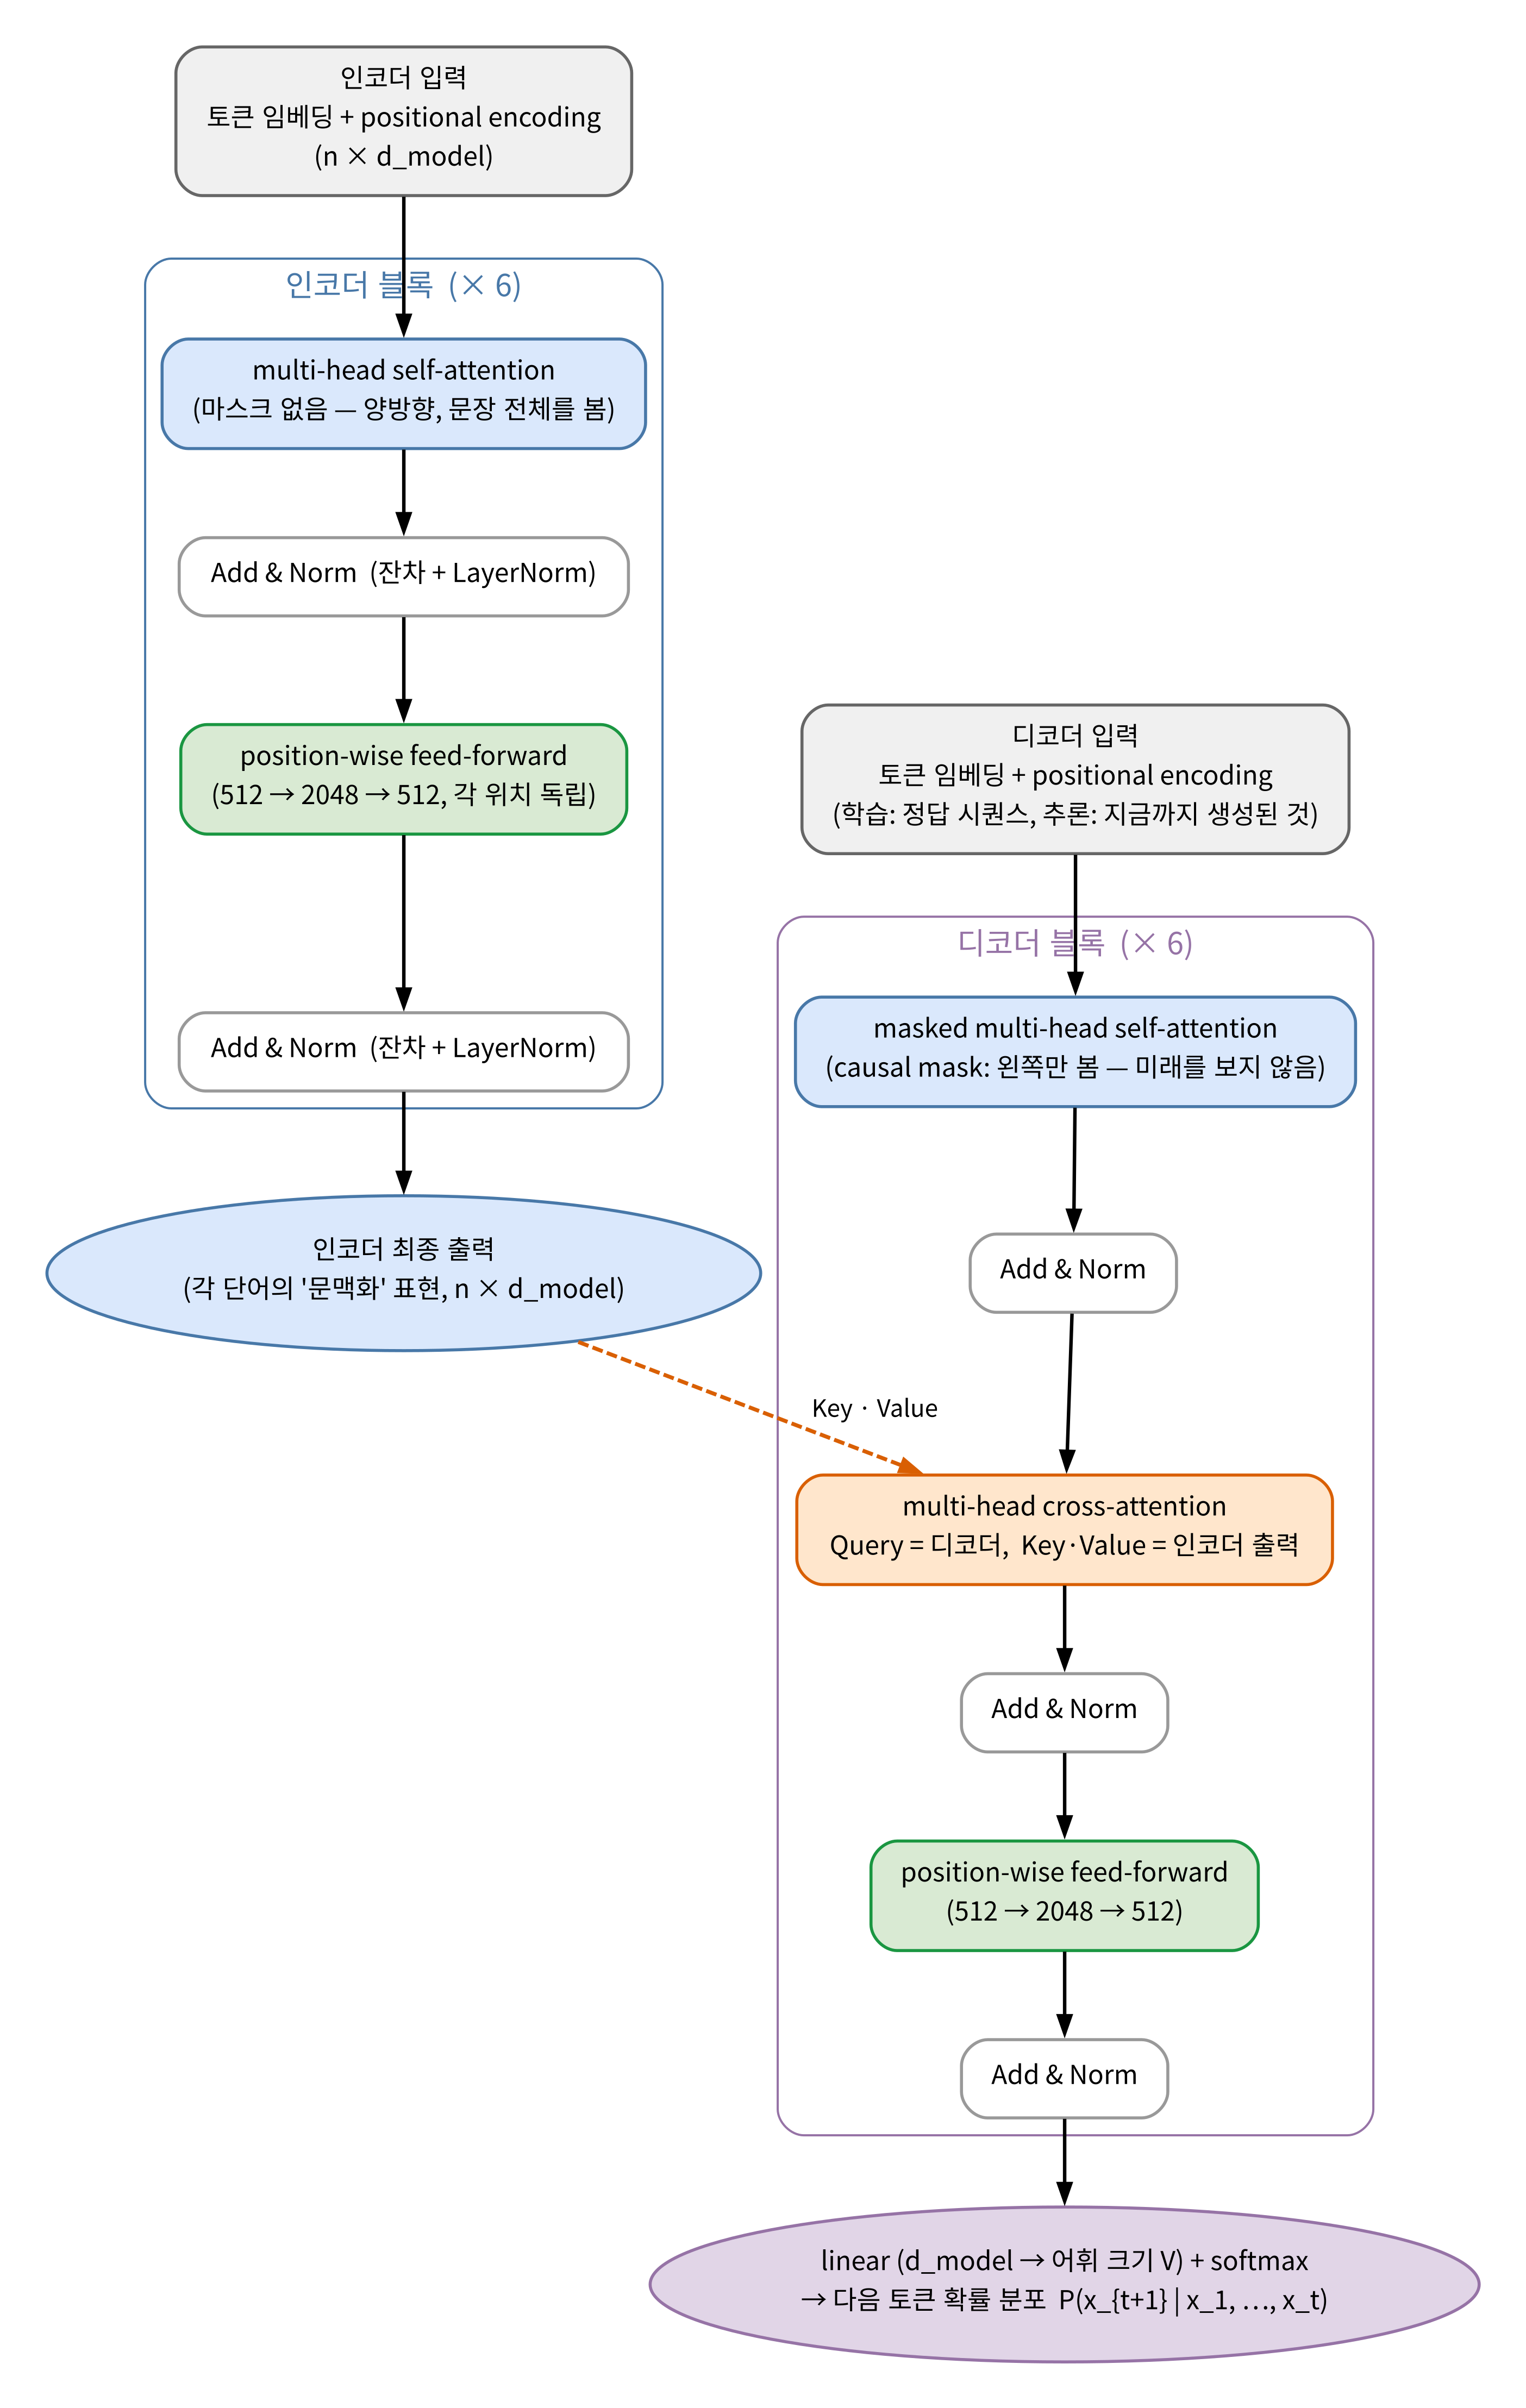
\includegraphics[width=0.72\linewidth]{ch12_3_transformer_block.png}
  \end{center}
  {\footnotesize 인코더 블록 = MHA + FFN(각각 Add\&Norm),
  6회 쌓기. 디코더 블록 = masked self-attention +
  cross-attention(인코더 출력) + FFN, 6회 쌓기. 입력/출력
  임베딩에 PE를 더하고, 디코더 출력은 linear + softmax로
  \textbf{토큰 확률 분포}를 낸다.}
\end{frame}

\begin{frame}{왜 attention 뒤에 FFN이 필요한가}
  \begin{itemize}
    \item self-attention은 \emph{단어 \emph{사이}의 정보를
      \emph{섞는}} 연산이지만, 그 연산 자체는 \textbf{선형}이다
      — 점수 $QK^T$, 가중합 $AV$ 모두 \textbf{선형} (Ch.\,9.2
      ``\textbf{선형만으로는 접을 수 없다}'' 기억하자).
    \item \emph{섞은 결과}에 \textbf{비선형 변환}을 적용하는
      역할이 \textbf{FFN의 몫}.
  \end{itemize}
  \vskip0.5em
  \begin{block}{분담}
    \textbf{attention} = ``\textbf{어떤 정보를, 어떤 단어끼리,
    얼마나 섞을지}'',
    그 뒤의 \textbf{FFN} = ``\textbf{섞인 정보를 어떻게
    \emph{처리}할지}'' — 9장 이후 반복된 \textbf{``선형 +
    비선형''} 논리의 또 다른 실체.
  \end{block}
  \vskip0.4em
  \begin{block}{참고: 파라미터 스케일의 감각}
    base 모델($d_{model}=512$, 6 블록)에서 한 블록의 파라미터
    대부분은 attention(QKV$+W_O$ 합계 약 \textbf{39만})보다
    \textbf{FFN}이 차지 — $512 \to 2048 \to 512 =
    2 \times 512 \times 2048 \approx$ \textbf{210만}.
    ``\textbf{트랜스포머의 지식이 어디에 있는지}''를 찾는 연구
    (FFN을 ``키-값 메모리''로 본 해석 — Geva et al., 2020)에서
    \textbf{사실상의 대부분이 FFN의 가중치에 담겨 있다}는
    관찰이 이 비율과 맞닿아 있다.
  \end{block}
\end{frame}

\begin{frame}{RNN 대비 이점}
  Self-attention은 \textbf{모든 단어 쌍을 \emph{한 번에} 병렬로}
  계산 — 순차 처리가 없어 \textbf{GPU 병렬성을 최대한 활용},
  ``1번째와 100번째 단위의 관련성''도 \textbf{중간 99단계를
  거치지 않고 직접} 계산(그래디언트 소실 문제 구조적으로
  훨씬 덜함).
  \vskip0.4em
  \textbf{대신}: 문장 길이의 \textbf{제곱}에 비례하는 계산량
  ($QK^T$ 가 $n \times n$ 행렬)이라는 \textbf{새로운 비용} —
  아주 긴 문서를 다룰 때의 실무적 한계.
  \small
  \begin{tabular}{@{}p{3.6cm}p{4.3cm}p{5.6cm}@{}}
    \toprule
    관점 & RNN/LSTM (Ch.11) & Self-Attention (Ch.12) \\
    \midrule
    1번째 $\to$ 100번째 단어 경로 & 99 단계(순차 언폴딩) &
      \textbf{1 단계}($Q\cdot K$ 직접) \\
    병렬성 & 없음(순차 필수) & \textbf{모든 쌍 동시} \\
    긴 거리 의존 & BPTT로 그래디언트 소실 & \textbf{구조적으로
      없음}(경로 항상 1) \\
    계산 복잡도(길이 $n$에 대해) & $O(n \cdot d^2)$ (선형) &
      $O(n^2 \cdot d)$ (\textbf{제곱}) \\
    순서 정보 & \emph{암묵적}(순차 구조 자체가) & \emph{명시적}
      (PE를 입력에 추가) \\
    \bottomrule
  \end{tabular}
\end{frame}

\begin{frame}{마지막 행이 앞 네 행의 ``대가(trade-off)''}
  \begin{itemize}
    \item 병렬성과 경로 길이 이점을 \emph{사면}, \textbf{그
      대가로}:
      \begin{enumerate}
        \item \textbf{제곱 계산량} ($O(n^2)$),
        \item ``\textbf{순서를 \emph{스스로} 인코딩}해야
          하는'' PE라는 \textbf{명시적 장치}.
      \end{enumerate}
    \item \textbf{RNN}은 \textbf{순서 정보를 \emph{계산 구조
      안에} 숨겼고}(대가: 순차성 + 소실), \textbf{어텐션}은
      \textbf{\emph{입력 안에} 넣었다}(대가: $n^2$ + PE 설계).
    \item 두 구조는 \textbf{같은 ``순서'' 정보를 \emph{다를
      곳에} 둔 것}.
  \end{itemize}
  \vskip0.5em
  \begin{block}{자주 묻는 질문 1: $O(n^2)$ 가 실전에서 얼마나}
    문장 1,000단어면 $1000^2 = 100\text{만}$ 쌍, 10,000단어면
    $1\text{억}$ 쌍 — \textbf{길이가 10배 늘면 계산량은 100배}.
    이 때문에 아주 긴 문서(책 한 권 분량)를 다루는 LLM은
    이 제곱 비용을 줄이는 \textbf{다양한 근사 기법}(희소
    어텐션 — Child et al., 2019; 슬라이딩 윈도우 등)을
    \emph{함께} 쓴다.
  \end{block}
\end{frame}

\begin{frame}{FAQ 3개: PE와 헤드, RNN 메모리}
  \begin{itemize}
    \item \kb{PE가 고정인데, 모델은 ``위치''를 실제로 \emph{배우는}
      건가?} 학습되는 것은 \emph{PE의 형태}가 아니라
      \emph{PE를 \emph{활용}할 방법}. PE는 ``\textbf{지도에
      좌표를 찍어 주는} 고정 장치''이고, 모델이 학습하는 것은
      ``\emph{좌표가 이런(상대) 관계로 다를 때 어텐션 점수를
      이렇게 준다}''는 \emph{가중치}($W_Q, W_K, W_O$ 안의
      패턴). \textbf{``PE는 고정, \emph{PE를 쓰는 가중치}가
      학습''}이라는 구분이 핵심.
    \item \kb{512로 학습한 모델이 1000 길이를 \emph{자동} 처리?}
      \textbf{아니다} — ``정의된다''는 \emph{PE 벡터 자체}가
      $t>512$ 에서도 \emph{유효한(비 NaN) 숫자}를 낸다는 뜻이지,
      \emph{그 위치에서의 어텐션 동작}이 학습되었다는 뜻은
      \emph{아니다}. \textbf{실제 ``장문 컨텍스트'' LLM}(LLaMA-2
      4K, GPT-4 128K 등)은 단순 PE 외삽이 \emph{아니라}
      \emph{추가 학습}(위치 보간 — Chen et al., 2023; 컨텍스트
      연장 미세조정 등)이 필요. \textbf{``함수가 정의된다''와
      ``동작이 학습된다''는 \emph{서로 다른} 두 문장}.
    \item \kb{어텐션이 대체한 것은 RNN의 ``메모리''인가?}
      RNN 은닉 상태 = \emph{순차 압축}된 ``과거 요약''.
      어텐션 = \emph{\textbf{압축이 아닌 랜덤 접근}}:
      \emph{모든} 과거(과 미래, mask 없으면)에 \emph{직접}
      접근. ``과거를 \emph{담아 두는} 메모리''(RNN 은닉
      상태)와 ``과거에 \emph{임의로 접근하는} 메커니즘''
      (어텐션)은 \emph{다른} 두 장치 — 어텐션이 \emph{더 좋은}
      것: (1) GPU 병렬성, (2) 경로 길이($\to$ 소실).
  \end{itemize}
\end{frame}

% ===== wrap-up =====
\begin{frame}{12주차 정리}
  \begin{enumerate}
    \item \kb{12.1 — 어텐션은 RNN의 패치에서 시작}
      압축 병목을 우회해 ``원문 전체를 다시 보고 적절한 비율로
      쓴다''. Q·K·V는 \emph{같은 입력에서 서로 다른} 세 변환 —
      $W_Q, W_K, W_V$ 가 \textbf{학습으로 결정}되며, 이 세
      행렬의 존재가 어텐션의 핵심.
    \item \kb{12.2 — 4단계와 $\sqrt{d_k}$}
      $QK^T \to$ $\sqrt{d_k}$ 스케일 $\to$ softmax $\to$
      $V$ 가중합. softmax는 \emph{원점수 차이를 지수적으로
      증폭}하고, $\sqrt{d_k}$ 는 \textbf{무작위 내적의 표준편차}
      (차원 $d_k$)를 1로 환원하는 상수 — one-hot으로 붙는
      softmax를 막는 안전장치.
    \item \kb{12.3 — 관점 $h$배 + 순서 명시적 인코딩}
      멀티헤드는 \textbf{파라미터를 재배분}해 독립 관점의
      수를 $h$배로 산다. PE는 시계(사인/코사인)의 \emph{회전
      성질}로 \emph{상대 위치}를 선형 도구로 읽게 해준다.
      causal mask가 \textbf{학습의 병렬성과 생성의 순차성}을
      하나로 통일.
  \end{enumerate}
  \vskip0.6em
  \begin{block}{다음 주차 — Chapter 13. 그래프 표현학습}
    노드와 엣지로 표현되는 데이터를 벡터로: Node2Vec·PageRank.
    ``어텐션이 단어 쌍의 관련성을 직접 계산''한다는 아이디어가
    ``그래프의 이웃 구조''로 이동한다.
  \end{block}
\end{frame}

\end{document}
